\documentclass{beamer}
\usepackage{etex}
\usepackage{pgfpages}

\usepackage{ifthen}

\providecommand{\NoExternal}{false}
\providecommand{\NoNotes}{true}

\ifthenelse{\equal{\NoNotes}{true}}{

}{
    \setbeameroption{show notes on second screen=right}
}
\makeatletter
\defbeamertemplate*{note page}{mynotes}
{%
  {%
    \scriptsize
    \usebeamerfont{note title}\usebeamercolor[fg]{note title}%
    \ifbeamercolorempty[bg]{note title}{}{%
      \insertvrule{.45\paperheight}{note title.bg}%
      \vskip-.45\paperheight%
      \nointerlineskip%
    }%
    \vbox{
      \hfill\insertslideintonotes{0.45}\hskip-\Gm@rmargin\hskip0pt%
      \vskip-0.45\paperheight%
      }
    \nointerlineskip
    \vbox to .45\paperheight{\vskip0.5em
      \hbox{\insertshorttitle[width=8cm]}%
      \setbox\beamer@tempbox=\hbox{\insertsection}%
      \hbox{\ifdim\wd\beamer@tempbox>1pt{\hskip4pt\raise3pt\hbox{\vrule
            width0.4pt height7pt\vrule width 9pt
            height0.4pt}}\hskip1pt\hbox{\begin{minipage}[t]{7.5cm}\def\breakhere{}\insertsection\end{minipage}}\fi%
      }%
      \setbox\beamer@tempbox=\hbox{\insertsubsection}%
      \hbox{\ifdim\wd\beamer@tempbox>1pt{\hskip17.4pt\raise3pt\hbox{\vrule
            width0.4pt height7pt\vrule width 9pt
            height0.4pt}}\hskip1pt\hbox{\begin{minipage}[t]{7.5cm}\def\breakhere{}\insertsubsection\end{minipage}}\fi%
      }%
      \setbox\beamer@tempbox=\hbox{\insertshortframetitle}%
      \hbox{\ifdim\wd\beamer@tempbox>1pt{\hskip30.8pt\raise3pt\hbox{\vrule
            width0.4pt height7pt\vrule width 9pt
            height0.4pt}}\hskip1pt\hbox{\insertshortframetitle[width=7cm]}\fi%
      }%
      \vfil
      \insertframenumber\,/\,\inserttotalframenumber}%
  }%
  \ifbeamercolorempty[bg]{note page}{}{%
    \nointerlineskip%
    \insertvrule{.55\paperheight}{note page.bg}%
    \vskip-.55\paperheight%
  }%
  \vskip.25em
  \nointerlineskip
  \insertnote
}
\makeatother

\setbeamertemplate{note page}[mynotes]

\title[FPGA based LP]{Diploma thesis}
\author[G.~Vormayr]{Gernot Vormayr\\0425210}
\institute[EMCE]{Institute of Electrodynamics, Microwave and Circuit Engineering}
\date[MW '15]{Microwave Engineering 2015}
\subtitle{FPGA based Load-Pull Measurement System}

\mode<presentation>
{
    \usetheme{CambridgeUS}
    \usecolortheme{dolphin} %whale?
    \usefonttheme{professionalfonts}
    \setbeamertemplate{navigation symbols}{}
}

%\AtBeginSubsection[]
%{
%  \begin{frame}<beamer>{Outline}
%    \tableofcontents[currentsection,currentsubsection]
%  \end{frame}
%}
\usepackage[overlay,absolute]{textpos}
\usepackage[english]{babel}

%drawings

\usepackage{graphicx}
\graphicspath{{images/}}
\usepackage{tikz}
\usepackage{circuitikz}
\usetikzlibrary{arrows.meta}
\usetikzlibrary{arrows}
\usetikzlibrary{backgrounds}
\usetikzlibrary{bending}
\usetikzlibrary{calc}
\usetikzlibrary{colorbrewer}
\usetikzlibrary{chains}
\usetikzlibrary{circuits.ee.IEC}
\usetikzlibrary{decorations.pathmorphing}
\usetikzlibrary{dsp}
\usetikzlibrary{fit}
\usetikzlibrary{matrix}
\usetikzlibrary{patterns}
\usetikzlibrary{positioning}
\usetikzlibrary{scopes}
\usetikzlibrary{shadows}
\usetikzlibrary{shapes.geometric}
\usetikzlibrary{shapes.misc}
\usepackage{tikz-timing}
\makeatletter

\ctikzset{rf/width/.initial=0.75}
\ctikzset{rf/height/.initial=0.75}
\ctikzset{rf/filter/sinewidth/.initial=0.8}
\ctikzset{rf/filter/sineheight/.initial=0.2}
\ctikzset{rf/switch/length/.initial=0.6}


\long\def\pgfrfdeclarenode#1#2#3{
    \pgfdeclareshape{#1}
    {
        \anchor{center}{
            \pgfpointorigin
        }
        \savedanchor\northwest{%
            \pgf@y=\pgfkeysvalueof{/tikz/circuitikz/bipoles/length}
            \pgf@y=\pgfkeysvalueof{/tikz/circuitikz/rf/height}\pgf@y
            \pgf@y=.5\pgf@y
            \pgf@x=\pgfkeysvalueof{/tikz/circuitikz/bipoles/length}
            \pgf@x=.5\pgf@x
            \pgf@x=-\pgfkeysvalueof{/tikz/circuitikz/rf/width}\pgf@x
        }
        \anchor{north}{
            \northwest
            \pgf@x=0pt
        }
        \anchor{south}{
            \northwest
            \pgf@x=0pt
            \pgf@y=-\pgf@y
        }
        \anchor{west}{
            \northwest
            \pgf@y=0pt
        }
        \anchor{east}{
            \northwest
            \pgf@y=0pt
            \pgf@x=-\pgf@x
        }
        \anchor{south west}{
            \northwest
            \pgf@y=-\pgf@y
        }
        \anchor{north east}{
            \northwest
            \pgf@x=-\pgf@x
        }
        \anchor{north west}{
            \northwest
        }
        \anchor{south east}{
            \northwest
            \pgf@x=-\pgf@x
            \pgf@y=-\pgf@y
        }	  
        \anchor{base}{
            \northwest
            \pgf@x=0pt	  	
        }
        \anchorborder{
            \@tempdima=\pgf@x
            \@tempdimb=\pgf@y
            \northwest
            \pgf@xa=-\pgf@x
            \pgf@ya=\pgf@y
            \pgfpointborderrectangle{\pgfpoint{\@tempdima}{\@tempdimb}}{\pgfpoint{\pgf@xa}{\pgf@ya}}
        }
        #3
        \backgroundpath{			
            \pgfsetcolor{\pgfkeysvalueof{/tikz/circuitikz/color}}	

            \northwest
            \pgf@circ@res@up = \pgf@y 
            \pgf@circ@res@down = -\pgf@y
            \pgf@circ@res@right = -\pgf@x
            \pgf@circ@res@left = \pgf@x

            \pgfscope
                \pgfsetcornersarced{\pgfpoint{4pt}{4pt}}
                \pgfpathrectanglecorners{\pgfpoint{\pgf@circ@res@left}{\pgf@circ@res@down}}{\pgfpoint{\pgf@circ@res@right}{\pgf@circ@res@up}}
                \pgfstroke
            \endpgfscope

            #2

        }
    }
}

\long\def\pgfrfdeclaresimplenode#1#2#3#4{
    \pgfdeclareshape{#1}
    {
        \anchor{center}{
            \pgfpointorigin
        }
        \savedanchor\northwest{%
            #2
        }
        \anchor{north}{
            \northwest
            \pgf@x=0pt
        }
        \anchor{south}{
            \northwest
            \pgf@x=0pt
            \pgf@y=-\pgf@y
        }
        \anchor{west}{
            \northwest
            \pgf@y=0pt
        }
        \anchor{east}{
            \northwest
            \pgf@y=0pt
            \pgf@x=-\pgf@x
        }
        \anchor{south west}{
            \northwest
            \pgf@y=-\pgf@y
        }
        \anchor{north east}{
            \northwest
            \pgf@x=-\pgf@x
        }
        \anchor{north west}{
            \northwest
        }
        \anchor{south east}{
            \northwest
            \pgf@x=-\pgf@x
            \pgf@y=-\pgf@y
        }	  
        \anchor{base}{
            \northwest
            \pgf@x=0pt	  	
        }
        #3
        \backgroundpath{			
            #4
        }
    }
}

\long\def\pgfrfdeclaredoublenode#1#2#3{
    \pgfdeclareshape{#1}
    {
        \anchor{center}{
            \pgfpointorigin
        }
        \savedanchor\northwest{%
            \pgf@y=\pgfkeysvalueof{/tikz/circuitikz/bipoles/length}
            \pgf@y=\pgfkeysvalueof{/tikz/circuitikz/rf/height}\pgf@y
            \pgf@y=.5\pgf@y
            \pgf@x=\pgfkeysvalueof{/tikz/circuitikz/bipoles/length}
            \pgf@x=.75\pgf@x
            \pgf@x=-\pgfkeysvalueof{/tikz/circuitikz/rf/width}\pgf@x
        }
        \anchor{north}{
            \northwest
            \pgf@x=0pt
        }
        \anchor{south}{
            \northwest
            \pgf@x=0pt
            \pgf@y=-\pgf@y
        }
        \anchor{west}{
            \northwest
            \pgf@y=0pt
        }
        \anchor{east}{
            \northwest
            \pgf@y=0pt
            \pgf@x=-\pgf@x
        }
        \anchor{south west}{
            \northwest
            \pgf@y=-\pgf@y
        }
        \anchor{north east}{
            \northwest
            \pgf@x=-\pgf@x
        }
        \anchor{north west}{
            \northwest
        }
        \anchor{south east}{
            \northwest
            \pgf@x=-\pgf@x
            \pgf@y=-\pgf@y
        }	  
        \anchor{base}{
            \northwest
            \pgf@x=0pt	  	
        }
        \anchorborder{
            \@tempdima=\pgf@x
            \@tempdimb=\pgf@y
            \northwest
            \pgf@xa=-\pgf@x
            \pgf@ya=\pgf@y
            \pgfpointborderrectangle{\pgfpoint{\@tempdima}{\@tempdimb}}{\pgfpoint{\pgf@xa}{\pgf@ya}}
        }
        #3
        \backgroundpath{			
            \pgfsetcolor{\pgfkeysvalueof{/tikz/circuitikz/color}}	

            \northwest
            \pgf@circ@res@up = \pgf@y 
            \pgf@circ@res@down = -\pgf@y
            \pgf@circ@res@right = -\pgf@x
            \pgf@circ@res@left = \pgf@x

            \pgfscope
                \pgfsetcornersarced{\pgfpoint{4pt}{4pt}}
                \pgfpathrectanglecorners{\pgfpoint{\pgf@circ@res@left}{\pgf@circ@res@down}}{\pgfpoint{\pgf@circ@res@right}{\pgf@circ@res@up}}
                \pgfstroke
            \endpgfscope

            #2

        }
    }
}

\long\def\pgfrfdeclaremonopole#1#2{
    \pgfrfdeclarenode{#1}{#2}{
        \anchor{A}{
            \northwest
            \pgf@y=0pt
        }
    }
}

\long\def\pgfrfdeclarebipole#1#2{
    \pgfrfdeclarenode{#1}{#2}{
        \anchor{A}{
            \northwest
            \pgf@y=0pt
        }
        \anchor{B}{
            \northwest
            \pgf@y=0pt
            \pgf@x=-\pgf@x
        }
    }
}

\long\def\pgfrfdeclarebipoleslash#1#2{
    \pgfrfdeclarebipole{#1}{
        \pgf@circ@res@step = \pgf@circ@res@left
        \pgfmathaddtolength{\pgf@circ@res@step}{4pt - 4pt*cos(-45)}
        \pgfpathmoveto{\pgfpoint{\pgf@circ@res@step}{\pgf@circ@res@step}}
        \pgfpathlineto{\pgfpoint{-\pgf@circ@res@step}{-\pgf@circ@res@step}}
        \pgfusepath{draw}
        #2
    }
}

\long\def\pgfrfdeclaretripole#1#2{
    \pgfrfdeclarenode{#1}{#2}{
        \anchor{A1}{
            \northwest
            \pgf@y=0pt
        }
        \anchor{B1}{
            \northwest
            \pgf@y=0.5\pgf@y
            \pgf@x=-\pgf@x
        }
        \anchor{B2}{
            \northwest
            \pgf@y=-0.5\pgf@y
            \pgf@x=-\pgf@x
        }
    }
}

\long\def\pgfrfdeclarequadpole#1#2{
    \pgfrfdeclarenode{#1}{#2}{
        \anchor{A1}{
            \northwest
            \pgf@y=0.5\pgf@y
        }
        \anchor{A2}{
            \northwest
            \pgf@y=-0.5\pgf@y
        }
        \anchor{B1}{
            \northwest
            \pgf@y=0.5\pgf@y
            \pgf@x=-\pgf@x
        }
        \anchor{B2}{
            \northwest
            \pgf@y=-0.5\pgf@y
            \pgf@x=-\pgf@x
        }
    }
}

\pgfrfdeclarebipole{attenuator}{
    \pgfscope             
        \pgftransformscale{.5}
        \pgfnode{resistorshape}{center}{}{pgf@att}{\pgfusepath{stroke}}
    \endpgfscope
    \pgfpathmoveto{\pgfpoint{\pgf@circ@res@left}{0}}
    \pgfpathlineto{\pgfpointanchor{pgf@att}{b}}
    \pgfpathmoveto{\pgfpoint{\pgf@circ@res@right}{0}}
    \pgfpathlineto{\pgfpointanchor{pgf@att}{a}}
    \pgfusepath{draw}

}

\pgfrfdeclarebipole{vattenuator}{
    \pgfscope             
        \pgftransformscale{.5}
        \pgfnode{resistorshape}{center}{}{pgf@att}{\pgfusepath{stroke}}
    \endpgfscope
    \pgfpathmoveto{\pgfpoint{\pgf@circ@res@left}{0}}
    \pgfpathlineto{\pgfpointanchor{pgf@att}{b}}
    \pgfpathmoveto{\pgfpoint{\pgf@circ@res@right}{0}}
    \pgfpathlineto{\pgfpointanchor{pgf@att}{a}}
    \pgfusepath{draw}
    \pgfpathmoveto{\pgfpoint{0.5\pgf@circ@res@left}{0.7\pgf@circ@res@down}}
    \pgfpathlineto{\pgfpoint{0.5\pgf@circ@res@right}{0.7\pgf@circ@res@up}}
    \pgfsetarrowsend{stealth}
    \pgfusepath{draw}
}

\def\pgfrffiltersinewave{
        \pgfpathmoveto{\pgfpoint{\pgf@xb}{\pgf@yb}}
        \pgfpathsine{\pgfpoint{\pgf@xa}{\pgf@ya}}
        \pgfpathcosine{\pgfpoint{\pgf@xa}{-\pgf@ya}}
        \pgfpathsine{\pgfpoint{\pgf@xa}{-\pgf@ya}}
        \pgfpathcosine{\pgfpoint{\pgf@xa}{\pgf@ya}}
        \advance \pgf@yb by \pgf@circ@res@step
}

\long\def\pgfrfdeclarefilter#1#2{
    \pgfrfdeclarebipole{#1}{
        \pgfscope
            \pgf@yb = 0.5\pgf@circ@res@up
            \pgf@circ@res@step = -0.5\pgf@circ@res@up
            
            \pgf@xa = \ctikzvalof{rf/filter/sinewidth}\pgf@circ@res@right
            \divide \pgf@xa by 2
            \pgf@ya = \ctikzvalof{rf/filter/sineheight}\pgf@circ@res@up
            \pgf@xb = \ctikzvalof{rf/filter/sinewidth}\pgf@circ@res@left

            \pgfrffiltersinewave
            \pgfrffiltersinewave
            \pgfrffiltersinewave
            \pgfstroke
        \endpgfscope
        #2
    }
}

\def\pgfrfstrikewave#1{
    \pgf@ya = 0.5\pgf@circ@res@up
    \pgf@yb = #1\pgf@ya
    \advance \pgf@ya by -\pgf@yb
    \advance \pgf@ya by -2pt
    \pgfpathmoveto{\pgfpoint{-2pt}{\pgf@ya}}
    \advance \pgf@ya by 4pt
    \pgfpathlineto{\pgfpoint{2pt}{\pgf@ya}}
}

\pgfrfdeclarefilter{lowpass}{
    \pgfrfstrikewave{0}
    \pgfrfstrikewave{1}
    \pgfusepath{draw}
}

\pgfrfdeclarefilter{highpass}{
    \pgfrfstrikewave{1}
    \pgfrfstrikewave{2}
    \pgfusepath{draw}
}

\pgfrfdeclarefilter{bandpass}{
    \pgfrfstrikewave{0}
    \pgfrfstrikewave{2}
    \pgfusepath{draw}
}

\pgfrfdeclarefilter{allpass}{
}

\pgfrfdeclaretripole{altswitch}{
    \pgf@xa = \ctikzvalof{rf/switch/length}\pgf@circ@res@left
    \pgfpathmoveto{\pgfpoint{\pgf@circ@res@left}{0}}
    \pgfpathlineto{\pgfpoint{\pgf@xa}{0}}
    \pgfpathlineto{\pgfpoint{-\pgf@xa}{-0.5\pgf@circ@res@up}}
    \pgfpathlineto{\pgfpoint{\pgf@circ@res@right}{-0.5\pgf@circ@res@up}}
    \pgfpathmoveto{\pgfpoint{\pgf@circ@res@right}{0.5\pgf@circ@res@up}}
    \pgfpathlineto{\pgfpoint{-\pgf@xa}{0.5\pgf@circ@res@up}}
    \pgfusepath{draw}
    \pgfpathcircle{\pgfpoint{-\ctikzvalof{rf/switch/length}\pgf@circ@res@left}{-0.5\pgf@circ@res@up}}{1.5pt}
    \pgfusepath{draw,fill}
    \pgfsetfillcolor{white}
    \pgfpathcircle{\pgfpoint{-\ctikzvalof{rf/switch/length}\pgf@circ@res@left}{0.5\pgf@circ@res@up}}{1.5pt}
    \pgfusepath{draw,fill}
    \pgfpathmoveto{\pgfpoint{0}{0.25\pgf@circ@res@down}}
    \pgfmathsetmacro{\tikz@start@angle@temp}{(atan2(0.5*\the\pgf@circ@res@up,2*\ctikzvalof{rf/switch/length}*\the\pgf@circ@res@right))}
    \pgfpatharc{-\tikz@start@angle@temp}{+\tikz@start@angle@temp}{\ctikzvalof{rf/switch/length}\pgf@circ@res@right}
    \pgfsetarrowsend{stealth}
    \pgfusepath{draw}
}

\pgfrfdeclarequadpole{chswitch}{
    \pgf@xa = \ctikzvalof{rf/switch/length}\pgf@circ@res@left
    \pgfpathmoveto{\pgfpoint{\pgf@circ@res@left}{0.5\pgf@circ@res@up}}
    \pgfpathlineto{\pgfpoint{\pgf@circ@res@right}{0.5\pgf@circ@res@up}}
    \pgfpathmoveto{\pgfpoint{\pgf@circ@res@left}{0.5\pgf@circ@res@down}}
    \pgfpathlineto{\pgfpoint{\pgf@circ@res@right}{0.5\pgf@circ@res@down}}
    \pgfusepath{draw}
    \pgfpathmoveto{\pgfpoint{\ctikzvalof{rf/switch/length}\pgf@circ@res@left}{0.5\pgf@circ@res@up}}{1.5pt}
    \pgfpathlineto{\pgfpoint{\ctikzvalof{rf/switch/length}\pgf@circ@res@right}{0.5\pgf@circ@res@down}}{1.5pt}
    \pgfpathmoveto{\pgfpoint{\ctikzvalof{rf/switch/length}\pgf@circ@res@right}{0.5\pgf@circ@res@up}}{1.5pt}
    \pgfpathlineto{\pgfpoint{\ctikzvalof{rf/switch/length}\pgf@circ@res@left}{0.5\pgf@circ@res@down}}{1.5pt}
    \pgfsetdash{{3pt}{2pt}}{0pt}
    \pgfusepath{draw}
    \pgfsetfillcolor{white}
    \pgfsetdash{}{0pt}
    \pgfpathcircle{\pgfpoint{\ctikzvalof{rf/switch/length}\pgf@circ@res@left}{0.5\pgf@circ@res@up}}{1.5pt}
    \pgfpathcircle{\pgfpoint{\ctikzvalof{rf/switch/length}\pgf@circ@res@left}{0.5\pgf@circ@res@down}}{1.5pt}
    \pgfpathcircle{\pgfpoint{\ctikzvalof{rf/switch/length}\pgf@circ@res@right}{0.5\pgf@circ@res@up}}{1.5pt}
    \pgfpathcircle{\pgfpoint{\ctikzvalof{rf/switch/length}\pgf@circ@res@right}{0.5\pgf@circ@res@down}}{1.5pt}
    \pgfusepath{draw,fill}
}

\pgfrfdeclarebipoleslash{adc}{
    \pgfscope
        \pgftransformshift{\pgfpoint{0.5\pgf@circ@res@left}{0.5\pgf@circ@res@up}}
        \pgftext{A}
    \endpgfscope
    \pgfscope
        \pgftransformshift{\pgfpoint{0.5\pgf@circ@res@right}{0.5\pgf@circ@res@down}}
        \pgftext{D}
    \endpgfscope
}

\pgfrfdeclarebipoleslash{dac}{
    \pgfscope
        \pgftransformshift{\pgfpoint{0.5\pgf@circ@res@left}{0.5\pgf@circ@res@up}}
        \pgftext{D}
    \endpgfscope
    \pgfscope
        \pgftransformshift{\pgfpoint{0.5\pgf@circ@res@right}{0.5\pgf@circ@res@down}}
        \pgftext{A}
    \endpgfscope
}

\pgfrfdeclarebipole{amp}{
    \pgfscope             
        \pgftransformscale{.5}
        \pgfnode{buffer}{center}{}{pgf@amp}{\pgfusepath{stroke}}
    \endpgfscope
    \pgfpathmoveto{\pgfpoint{\pgf@circ@res@left}{0}}
    \pgfpathlineto{\pgfpointanchor{pgf@amp}{in}}
    \pgfpathmoveto{\pgfpoint{\pgf@circ@res@right}{0}}
    \pgfpathlineto{\pgfpointanchor{pgf@amp}{out}}
    \pgfusepath{draw}
}

\pgfrfdeclaresimplenode{mixer}
{
    \pgf@y=\pgfkeysvalueof{/tikz/circuitikz/bipoles/length}
    \pgf@y=\pgfkeysvalueof{/tikz/circuitikz/tripoles/mixer/height}\pgf@y
    \pgf@y=.4\pgf@y
    \pgf@y=.5\pgf@y
    \pgf@x=\pgfkeysvalueof{/tikz/circuitikz/bipoles/length}
    \pgf@x=.5\pgf@x
    \pgf@x=.4\pgf@x
    \pgf@x=-\pgfkeysvalueof{/tikz/circuitikz/tripoles/mixer/width}\pgf@x
}
{
    \anchorborder{
        \@tempdima=\pgf@x
        \@tempdimb=\pgf@y
        \northwest
        \pgf@xa=-\pgf@x
        \pgf@ya=\pgf@y
        \pgfpointborderellipse{\pgfpoint{\@tempdima}{\@tempdimb}}{\pgfpoint{\pgf@xa}{\pgf@ya}}
    }
}
{
    \northwest
    \pgf@circ@res@up = \pgf@y 
    \pgf@circ@res@down = -\pgf@y
    \pgf@circ@res@right = -\pgf@x
    \pgf@circ@res@left = \pgf@x
    \pgfscope
        \pgfsetlinewidth{\pgfkeysvalueof{/tikz/circuitikz/bipoles/thickness}\pgflinewidth}
        \pgfpathcircle{\pgfpoint{0}{0}}{\pgf@circ@res@up}
        \pgfusepath{draw}
    \endpgfscope
    \pgfmathsetlength{\pgf@circ@res@step}{\the\pgf@circ@res@right*cos(45)}
    \pgfpathmoveto{\pgfpoint{\pgf@circ@res@step}{\pgf@circ@res@step}}
    \pgfpathlineto{\pgfpoint{-\pgf@circ@res@step}{-\pgf@circ@res@step}}
    \pgfpathmoveto{\pgfpoint{-\pgf@circ@res@step}{\pgf@circ@res@step}}
    \pgfpathlineto{\pgfpoint{\pgf@circ@res@step}{-\pgf@circ@res@step}}
    \pgfusepath{draw}
}


\pgfrfdeclarenode{iqmix}{
    \pgfscope             
        \pgftransformshift{\pgfpoint{0.5\pgf@circ@res@right}{0.5\pgf@circ@res@up}}
        \pgftransformrotate{180}
        \pgftransformscale{.2}
        \pgfnode{mixer}{center}{}{pgf@mixi}{\pgfusepath{stroke}}
    \endpgfscope
    \pgfscope             
        \pgftransformshift{\pgfpoint{0}{0.5\pgf@circ@res@down}}
        \pgftransformrotate{180}
        \pgftransformscale{.2}
        \pgfnode{mixer}{center}{}{pgf@mixq}{\pgfusepath{stroke}}
    \endpgfscope
    \pgfscope             
        \pgftransformscale{.35}
        \pgfnode{rectangle}{center}{$90\degree$}{pgf@phase}{\pgfusepath{stroke}}
    \endpgfscope
    \pgfpathmoveto{\pgfpoint{\pgf@circ@res@left}{0pt}}
    \pgfpathlineto{\pgfpoint{0.6\pgf@circ@res@left}{0pt}}
    \pgfpathlineto{\pgfpoint{0.6\pgf@circ@res@left}{0.5\pgf@circ@res@up}}
    \pgfpathlineto{\pgfpointanchor{pgf@mixi}{out}}
    \pgfpathmoveto{\pgfpoint{0.6\pgf@circ@res@left}{0pt}}
    \pgfpathlineto{\pgfpoint{0.6\pgf@circ@res@left}{0.5\pgf@circ@res@down}}
    \pgfpathlineto{\pgfpointanchor{pgf@mixq}{out}}
    \pgfpathmoveto{\pgfpointanchor{pgf@mixi}{in}}
    \pgfpathlineto{\pgfpoint{\pgf@circ@res@right}{0.5\pgf@circ@res@up}}
    \pgfpathmoveto{\pgfpointanchor{pgf@mixq}{in}}
    \pgfpathlineto{\pgfpoint{\pgf@circ@res@right}{0.5\pgf@circ@res@down}}
    \pgfpathmoveto{\pgfpoint{0pt}{\pgf@circ@res@up}}
    \pgfpathlineto{\pgfpointanchor{pgf@phase}{north}}
    \pgfpathmoveto{\pgfpointanchor{pgf@phase}{south}}
    \pgfpathlineto{\pgfpointanchor{pgf@mixq}{in 2}}
    \pgfpathmoveto{\pgfpoint{0pt}{0.8\pgf@circ@res@up}}
    \pgfpathlineto{\pgfpoint{0.5\pgf@circ@res@right}{0.8\pgf@circ@res@up}}
    \pgfpathlineto{\pgfpointanchor{pgf@mixi}{in 2}}
    \pgfusepath{draw}
    \pgfpathcircle{\pgfpoint{0pt}{0.8\pgf@circ@res@up}}{1pt}
    \pgfpathcircle{\pgfpoint{0.6\pgf@circ@res@left}{0pt}}{1pt}
    \pgfusepath{fill}

}{
    \anchor{A1}{
        \northwest
        \pgf@y=0pt
    }
    \anchor{B1}{
        \northwest
        \pgf@y=0.5\pgf@y
        \pgf@x=-\pgf@x
    }
    \anchor{B2}{
        \northwest
        \pgf@y=-0.5\pgf@y
        \pgf@x=-\pgf@x
    }
    \anchor{C1}{
        \northwest
        \pgf@x=0pt
    }
}

\pgfrfdeclarenode{iqmixdown}{
    \pgfscope             
        \pgftransformshift{\pgfpoint{0.5\pgf@circ@res@right}{0.5\pgf@circ@res@down}}
        \pgftransformscale{.2}
        \pgfnode{mixer}{center}{}{pgf@mixi}{\pgfusepath{stroke}}
    \endpgfscope
    \pgfscope             
        \pgftransformshift{\pgfpoint{0}{0.5\pgf@circ@res@up}}
        \pgftransformscale{.2}
        \pgfnode{mixer}{center}{}{pgf@mixq}{\pgfusepath{stroke}}
    \endpgfscope
    \pgfscope             
        \pgftransformscale{.35}
        \pgfnode{rectangle}{center}{$90\degree$}{pgf@phase}{\pgfusepath{stroke}}
    \endpgfscope
    \pgfpathmoveto{\pgfpoint{\pgf@circ@res@left}{0pt}}
    \pgfpathlineto{\pgfpoint{0.6\pgf@circ@res@left}{0pt}}
    \pgfpathlineto{\pgfpoint{0.6\pgf@circ@res@left}{0.5\pgf@circ@res@down}}
    \pgfpathlineto{\pgfpointanchor{pgf@mixi}{in}}
    \pgfpathmoveto{\pgfpoint{0.6\pgf@circ@res@left}{0pt}}
    \pgfpathlineto{\pgfpoint{0.6\pgf@circ@res@left}{0.5\pgf@circ@res@up}}
    \pgfpathlineto{\pgfpointanchor{pgf@mixq}{in}}
    \pgfpathmoveto{\pgfpointanchor{pgf@mixi}{out}}
    \pgfpathlineto{\pgfpoint{\pgf@circ@res@right}{0.5\pgf@circ@res@down}}
    \pgfpathmoveto{\pgfpointanchor{pgf@mixq}{out}}
    \pgfpathlineto{\pgfpoint{\pgf@circ@res@right}{0.5\pgf@circ@res@up}}
    \pgfpathmoveto{\pgfpoint{0pt}{\pgf@circ@res@down}}
    \pgfpathlineto{\pgfpointanchor{pgf@phase}{south}}
    \pgfpathmoveto{\pgfpointanchor{pgf@phase}{north}}
    \pgfpathlineto{\pgfpointanchor{pgf@mixq}{in 2}}
    \pgfpathmoveto{\pgfpoint{0pt}{0.8\pgf@circ@res@down}}
    \pgfpathlineto{\pgfpoint{0.5\pgf@circ@res@right}{0.8\pgf@circ@res@down}}
    \pgfpathlineto{\pgfpointanchor{pgf@mixi}{in 2}}
    \pgfusepath{draw}
    \pgfpathcircle{\pgfpoint{0pt}{0.8\pgf@circ@res@down}}{1pt}
    \pgfpathcircle{\pgfpoint{0.6\pgf@circ@res@left}{0pt}}{1pt}
    \pgfusepath{fill}

}{
    \anchor{A1}{
        \northwest
        \pgf@y=0pt
    }
    \anchor{B1}{
        \northwest
        \pgf@y=0.5\pgf@y
        \pgf@x=-\pgf@x
    }
    \anchor{B2}{
        \northwest
        \pgf@y=-0.5\pgf@y
        \pgf@x=-\pgf@x
    }
    \anchor{C1}{
        \northwest
        \pgf@x=0pt
        \pgf@y=-\pgf@y
    }
}

\pgfrfdeclarebipole{pll}{
    \pgftext{PLL}
}

\pgfrfdeclarebipole{dut}{
    \pgftext{DUT}
}

\pgfrfdeclarebipole{vna}{
    \pgftext{VNA}
}

\pgfrfdeclarebipole{empty}{
}

\pgfrfdeclaresimplenode{source}
{
    \pgf@y=\pgfkeysvalueof{/tikz/circuitikz/bipoles/length}
    \pgf@y=\pgfkeysvalueof{/tikz/circuitikz/bipoles/vsource/height}\pgf@y
    \pgf@y=.5\pgf@y
    \pgf@x=\pgfkeysvalueof{/tikz/circuitikz/bipoles/length}
    \pgf@x=.5\pgf@x
    \pgf@x=-\pgfkeysvalueof{/tikz/circuitikz/bipoles/vsource/width}\pgf@x
}
{
    \anchorborder{
        \@tempdima=\pgf@x
        \@tempdimb=\pgf@y
        \northwest
        \pgf@xa=-\pgf@x
        \pgf@ya=\pgf@y
        \pgfpointborderellipse{\pgfpoint{\@tempdima}{\@tempdimb}}{\pgfpoint{\pgf@xa}{\pgf@ya}}
    }
}
{
    \northwest
    \pgf@circ@res@up = \pgf@y 
    \pgf@circ@res@down = -\pgf@y
    \pgf@circ@res@right = -\pgf@x
    \pgf@circ@res@left = \pgf@x
    \pgfscope             
        \pgftransformrotate{90}
        \pgfnode{vsourcesinshape}{center}{}{pgf@att}{\pgfusepath{stroke}}
    \endpgfscope
}

\pgfrfdeclaresimplenode{isolator}
{
    \pgf@y=\pgfkeysvalueof{/tikz/circuitikz/bipoles/length}
    \pgf@y=\pgfkeysvalueof{/tikz/circuitikz/bipoles/vsource/height}\pgf@y
    \pgf@y=.5\pgf@y
    \pgf@x=\pgfkeysvalueof{/tikz/circuitikz/bipoles/length}
    \pgf@x=.5\pgf@x
    \pgf@x=-\pgfkeysvalueof{/tikz/circuitikz/bipoles/vsource/width}\pgf@x
}
{
    \anchorborder{
        \@tempdima=\pgf@x
        \@tempdimb=\pgf@y
        \northwest
        \pgf@xa=-\pgf@x
        \pgf@ya=\pgf@y
        \pgfpointborderellipse{\pgfpoint{\@tempdima}{\@tempdimb}}{\pgfpoint{\pgf@xa}{\pgf@ya}}
    }
}
{
    \northwest
    \pgf@circ@res@up = \pgf@y 
    \pgf@circ@res@down = -\pgf@y
    \pgf@circ@res@right = -\pgf@x
    \pgf@circ@res@left = \pgf@x
    \pgfscope
        \pgfsetlinewidth{\pgfkeysvalueof{/tikz/circuitikz/bipoles/thickness}\pgflinewidth}
        \pgfpathcircle{\pgfpoint{0}{0}}{\pgf@circ@res@up}
        \pgfusepath{draw}
        \pgfsetarrowsend{latex}
        \pgfpathmoveto{\pgfpoint{0.8\pgf@circ@res@left}{0pt}}
        \pgfpathlineto{\pgfpoint{0.8\pgf@circ@res@right}{0pt}}
        \pgfusepath{draw}
    \endpgfscope
}

\pgfrfdeclaresimplenode{vphase}
{
    \pgf@y=\pgfkeysvalueof{/tikz/circuitikz/bipoles/length}
    \pgf@y=\pgfkeysvalueof{/tikz/circuitikz/bipoles/vsource/height}\pgf@y
    \pgf@y=.5\pgf@y
    \pgf@x=\pgfkeysvalueof{/tikz/circuitikz/bipoles/length}
    \pgf@x=.5\pgf@x
    \pgf@x=-\pgfkeysvalueof{/tikz/circuitikz/bipoles/vsource/width}\pgf@x
}
{
    \anchorborder{
        \@tempdima=\pgf@x
        \@tempdimb=\pgf@y
        \northwest
        \pgf@xa=-\pgf@x
        \pgf@ya=\pgf@y
        \pgfpointborderellipse{\pgfpoint{\@tempdima}{\@tempdimb}}{\pgfpoint{\pgf@xa}{\pgf@ya}}
    }
}
{
    \northwest
    \pgf@circ@res@up = \pgf@y 
    \pgf@circ@res@down = -\pgf@y
    \pgf@circ@res@right = -\pgf@x
    \pgf@circ@res@left = \pgf@x
    \pgfscope
        \pgfsetlinewidth{\pgfkeysvalueof{/tikz/circuitikz/bipoles/thickness}\pgflinewidth}
        \pgfpathcircle{\pgfpoint{0}{0}}{\pgf@circ@res@up}
        \pgfusepath{draw}
    \endpgfscope
    \pgfscope
        \pgfsetarrowsend{latex}
        \pgfpathmoveto{\pgfpoint{\pgf@circ@res@right}{\pgf@circ@res@up}}
        \pgfpathlineto{\pgfpoint{\pgf@circ@res@left}{\pgf@circ@res@down}}
        \pgfusepath{draw}
    \endpgfscope
}

\pgfrfdeclaresimplenode{tuner}
{
    \pgf@y=\pgfkeysvalueof{/tikz/circuitikz/bipoles/length}
    \pgf@y=\pgfkeysvalueof{/tikz/circuitikz/bipoles/tgeneric/height}\pgf@y
    \pgf@y=.5\pgf@y
    \pgf@x=\pgfkeysvalueof{/tikz/circuitikz/bipoles/length}
    \pgf@x=.5\pgf@x
    \pgf@x=-\pgfkeysvalueof{/tikz/circuitikz/bipoles/tgeneric/width}\pgf@x
}
{
    \anchorborder{
        \@tempdima=\pgf@x
        \@tempdimb=\pgf@y
        \northwest
        \pgf@xa=-\pgf@x
        \pgf@ya=\pgf@y
        \pgfpointborderrectangle{\pgfpoint{\@tempdima}{\@tempdimb}}{\pgfpoint{\pgf@xa}{\pgf@ya}}
    }
}
{
    \northwest
    \pgf@circ@res@up = \pgf@y 
    \pgf@circ@res@down = -\pgf@y
    \pgf@circ@res@right = -\pgf@x
    \pgf@circ@res@left = \pgf@x
    \pgfscope             
        \pgfnode{tgenericshape}{center}{}{pgf@att}{\pgfusepath{stroke}}
    \endpgfscope
}

\pgfrfdeclaresimplenode{amplifier}
{
    \pgf@y=\pgfkeysvalueof{/tikz/circuitikz/bipoles/length}
    \pgf@y=\pgfkeysvalueof{/tikz/circuitikz/bipoles/buffer/height}\pgf@y
    \pgf@y=.5\pgf@y
    \pgf@y=.6\pgf@y
    \pgf@x=\pgfkeysvalueof{/tikz/circuitikz/bipoles/length}
    \pgf@x=.5\pgf@x
    \pgf@x=.4\pgf@x
    \pgf@x=-\pgfkeysvalueof{/tikz/circuitikz/bipoles/buffer/width}\pgf@x
}
{
    \anchorborder{
        \@tempdima=\pgf@x
        \@tempdimb=\pgf@y
        \northwest
        \pgf@xa=-\pgf@x
        \pgf@ya=\pgf@y
        \pgfpointborderrectangle{\pgfpoint{\@tempdima}{\@tempdimb}}{\pgfpoint{\pgf@xa}{\pgf@ya}}
    }
}
{
    \northwest
    \pgf@circ@res@up = \pgf@y 
    \pgf@circ@res@down = -\pgf@y
    \pgf@circ@res@right = -\pgf@x
    \pgf@circ@res@left = \pgf@x
    \pgfscope
        \pgfsetlinewidth{\pgfkeysvalueof{/tikz/circuitikz/bipoles/thickness}\pgflinewidth}
        \pgfpathmoveto{\pgfpoint{\pgf@circ@res@left}{0pt}}
        \pgfpathlineto{\pgfpoint{\pgf@circ@res@right}{\pgf@circ@res@up}}
        \pgfpathlineto{\pgfpoint{\pgf@circ@res@right}{\pgf@circ@res@down}}
        \pgfpathclose
        \pgfusepath{stroke}
    \endpgfscope
}

\pgfrfdeclaresimplenode{match}
{
    \pgf@y=\pgfkeysvalueof{/tikz/circuitikz/bipoles/length}
    \pgf@y=\pgfkeysvalueof{/tikz/circuitikz/bipoles/resistor/height}\pgf@y
    \pgf@y=.5\pgf@y
    \pgf@x=\pgfkeysvalueof{/tikz/circuitikz/bipoles/length}
    \pgf@x=.5\pgf@x
    \pgf@x=-\pgfkeysvalueof{/tikz/circuitikz/bipoles/resistor/width}\pgf@x
}
{
    \anchorborder{
        \@tempdima=\pgf@x
        \@tempdimb=\pgf@y
        \northwest
        \pgf@xa=-\pgf@x
        \pgf@ya=\pgf@y
        \pgfpointborderrectangle{\pgfpoint{\@tempdima}{\@tempdimb}}{\pgfpoint{\pgf@xa}{\pgf@ya}}
    }
}
{
    \northwest
    \pgf@circ@res@up = \pgf@y 
    \pgf@circ@res@down = -\pgf@y
    \pgf@circ@res@right = -\pgf@x
    \pgf@circ@res@left = \pgf@x
    \pgfscope             
        \pgfnode{resistorshape}{center}{}{pgf@att}{\pgfusepath{stroke}}
    \endpgfscope
}

\pgfrfdeclaresimplenode{vmatch}
{
    \pgf@y=\pgfkeysvalueof{/tikz/circuitikz/bipoles/length}
    \pgf@y=\pgfkeysvalueof{/tikz/circuitikz/bipoles/vresistor/height}\pgf@y
    \pgf@y=.5\pgf@y
    \pgf@x=\pgfkeysvalueof{/tikz/circuitikz/bipoles/length}
    \pgf@x=.5\pgf@x
    \pgf@x=-\pgfkeysvalueof{/tikz/circuitikz/bipoles/vresistor/width}\pgf@x
}
{
    \anchorborder{
        \@tempdima=\pgf@x
        \@tempdimb=\pgf@y
        \northwest
        \pgf@xa=-\pgf@x
        \pgf@ya=\pgf@y
        \pgfpointborderrectangle{\pgfpoint{\@tempdima}{\@tempdimb}}{\pgfpoint{\pgf@xa}{\pgf@ya}}
    }
}
{
    \northwest
    \pgf@circ@res@up = \pgf@y 
    \pgf@circ@res@down = -\pgf@y
    \pgf@circ@res@right = -\pgf@x
    \pgf@circ@res@left = \pgf@x
    \pgfscope             
        \pgfnode{vresistorshape}{center}{}{pgf@att}{\pgfusepath{stroke}}
    \endpgfscope
}

\long\def\pgfrfdeclarecoupler#1#2{
    \pgfrfdeclaredoublenode{#1}{
        \pgfpathmoveto{\pgfpoint{\pgf@circ@res@left}{0pt}}
        \pgfpathlineto{\pgfpoint{\pgf@circ@res@right}{0pt}}
        \pgfusepath{draw}
        \pgf@xa = 0.75\pgf@circ@res@left
        \pgfscope
            \pgfsetlinewidth{1pt}
            \advance \pgf@xa by 4pt
            \pgfpathmoveto{\pgfpoint{\pgf@xa}{0pt}}
            \pgfpathlineto{\pgfpoint{-\pgf@xa}{0pt}}
            \pgfpathmoveto{\pgfpoint{\pgf@xa}{0.15\pgf@circ@res@up}}
            \pgfpathlineto{\pgfpoint{-\pgf@xa}{0.15\pgf@circ@res@up}}
            \pgfusepath{draw}
        \endpgfscope
        \pgfscope
            \pgfsetcornersarced{\pgfpoint{4pt}{4pt}}
            #2
            \pgfusepath{draw}
        \endpgfscope
    }{
        \anchor{A1}{
            \northwest
            \pgf@y=0pt
        }
        \anchor{A2}{
            \northwest
            \pgf@x=0.75\pgf@x
        }
        \anchor{B1}{
            \northwest
            \pgf@x=-\pgf@x
            \pgf@y=0pt
        }
        \anchor{B2}{
            \northwest
            \pgf@x=-0.75\pgf@x
        }
    }
}

\pgfrfdeclarecoupler{dircoupler}{
    \pgfpathmoveto{\pgfpoint{0.75\pgf@circ@res@left}{\pgf@circ@res@up}}
    \pgfpathlineto{\pgfpoint{0.75\pgf@circ@res@left}{0.15\pgf@circ@res@up}}
    \pgfpathlineto{\pgfpoint{0.75\pgf@circ@res@right}{0.15\pgf@circ@res@up}}
    \pgfpathlineto{\pgfpoint{0.75\pgf@circ@res@right}{\pgf@circ@res@up}}
}

\pgfrfdeclarecoupler{dircouplera}{
    \pgfpathmoveto{\pgfpoint{0.75\pgf@circ@res@left}{\pgf@circ@res@up}}
    \pgfpathlineto{\pgfpoint{0.75\pgf@circ@res@left}{0.15\pgf@circ@res@up}}
    \pgfpathlineto{\pgfpoint{0pt}{0.15\pgf@circ@res@up}}
}

\pgfrfdeclarecoupler{dircouplerb}{
    \pgfpathmoveto{\pgfpoint{0.75\pgf@circ@res@left}{0.15\pgf@circ@res@up}}
    \pgfpathlineto{\pgfpoint{0.75\pgf@circ@res@right}{0.15\pgf@circ@res@up}}
    \pgfpathlineto{\pgfpoint{0pt}{0.15\pgf@circ@res@up}}
}

\pgfrfdeclaremonopole{generator}{
    \pgfscope             
        \pgftransformscale{.5}
        \pgftransformrotate{90}
        \pgfnode{vsourcesinshape}{center}{}{pgf@att}{\pgfusepath{stroke}}
    \endpgfscope
}

\pgfrfdeclaremonopole{powermeter}{
    \pgfscope             
        \pgftransformscale{.5}
        \pgftransformrotate{-90}
        \pgfnode{fulldiodeshape}{center}{}{pgf@att}{\pgfusepath{stroke}}
    \endpgfscope
    \pgfpathmoveto{\pgfpoint{0pt}{0.7\pgf@circ@res@up}}
    \pgfpathlineto{\pgfpoint{0pt}{0.7\pgf@circ@res@down}}
    \pgfusepath{draw}
}

\pgfrfdeclaremonopole{spectrum analyzer}{
    \pgfpathmoveto{\pgfpoint{0.7\pgf@circ@res@down}{0.8\pgf@circ@res@left}}
    \pgfpathlineto{\pgfpoint{0.7\pgf@circ@res@down}{0.7\pgf@circ@res@right}}
    \pgfpathmoveto{\pgfpoint{0.8\pgf@circ@res@down}{0.7\pgf@circ@res@left}}
    \pgfpathlineto{\pgfpoint{0.7\pgf@circ@res@up}{0.7\pgf@circ@res@left}}
    \pgfusepath{draw}

    \pgfsetcornersarced{\pgfpoint{2pt}{1pt}}
    \pgfpathmoveto{\pgfpoint{0.7\pgf@circ@res@left}{0.6\pgf@circ@res@down}}
    \pgfpathlineto{\pgfpoint{0.55\pgf@circ@res@left}{0.6\pgf@circ@res@down}}
    \pgfpathlineto{\pgfpoint{0.5\pgf@circ@res@left}{0.4\pgf@circ@res@up}}
    \pgfpathlineto{\pgfpoint{0.45\pgf@circ@res@left}{0.6\pgf@circ@res@down}}
    \pgfpathlineto{\pgfpoint{0.05\pgf@circ@res@left}{0.6\pgf@circ@res@down}}
    \pgfpathlineto{\pgfpoint{0}{0.6\pgf@circ@res@up}}
    \pgfpathlineto{\pgfpoint{0.05\pgf@circ@res@right}{0.6\pgf@circ@res@down}}
    \pgfpathlineto{\pgfpoint{0.45\pgf@circ@res@right}{0.6\pgf@circ@res@down}}
    \pgfpathlineto{\pgfpoint{0.5\pgf@circ@res@right}{0.4\pgf@circ@res@up}}
    \pgfpathlineto{\pgfpoint{0.55\pgf@circ@res@right}{0.6\pgf@circ@res@down}}
    \pgfpathlineto{\pgfpoint{0.7\pgf@circ@res@right}{0.6\pgf@circ@res@down}}
    \pgfusepath{draw}
}

\pgfrfdeclaretripole{splitter}{
    \pgfscope             
        \pgftransformshift{\pgfpoint{0.5\pgf@circ@res@right}{0}}
        \pgftransformscale{.2}
        \pgftransformrotate{-90}
        \pgfnode{resistorshape}{center}{}{pgf@att}{\pgfusepath{stroke}}
    \endpgfscope
    \pgfpathmoveto{\pgfpoint{\pgf@circ@res@left}{0}}
    \pgfpathlineto{\pgfpoint{.5\pgf@circ@res@left}{0}}
    \pgfpathlineto{\pgfpoint{.5\pgf@circ@res@right}{.5\pgf@circ@res@up}}
    \pgfpathlineto{\pgfpoint{\pgf@circ@res@right}{.5\pgf@circ@res@up}}
    \pgfpathmoveto{\pgfpoint{.5\pgf@circ@res@left}{0}}
    \pgfpathlineto{\pgfpoint{.5\pgf@circ@res@right}{.5\pgf@circ@res@down}}
    \pgfpathlineto{\pgfpoint{\pgf@circ@res@right}{.5\pgf@circ@res@down}}
    \pgfpathmoveto{\pgfpointanchor{pgf@att}{east}}
    \pgfpathlineto{\pgfpoint{.5\pgf@circ@res@right}{.5\pgf@circ@res@down}}
    \pgfpathmoveto{\pgfpointanchor{pgf@att}{west}}
    \pgfpathlineto{\pgfpoint{.5\pgf@circ@res@right}{.5\pgf@circ@res@up}}
    \pgfusepath{draw}
}

\pgfrfdeclarebipole{dc block}{
    \pgfscope             
        \pgftransformscale{.5}
        \pgfnode{capacitorshape}{center}{}{pgf@att}{\pgfusepath{stroke}}
    \endpgfscope
    \pgfpathmoveto{\pgfpoint{\pgf@circ@res@left}{0}}
    \pgfpathlineto{\pgfpointanchor{pgf@att}{b}}
    \pgfpathmoveto{\pgfpoint{\pgf@circ@res@right}{0}}
    \pgfpathlineto{\pgfpointanchor{pgf@att}{a}}
    \pgfusepath{draw}

}

\pgfrfdeclaredoublenode{oscilloscope}{
    \pgfscope
        \pgfsetcornersarced{\pgfpoint{2pt}{2pt}}
        \pgfpathrectanglecorners{\pgfpoint{0.9\pgf@circ@res@left}{0.4\pgf@circ@res@down}}{\pgfpoint{0.1\pgf@circ@res@left}{0.75\pgf@circ@res@up}}
        \pgfusepath{draw}
    \endpgfscope
    \foreach \posc/\post/\i in {0.2/0.15/4,0.4/0.35/3,0.6/0.55/2,0.8/0.75/1}{
        \pgfscope
            \pgftransformshift{\pgfpoint{\post\pgf@circ@res@left}{0.6\pgf@circ@res@down}}
            \pgftransformscale{.4}
            \pgftext{\i}
            \pgfusepath{draw}
        \endpgfscope
        \pgfpathcircle{\pgfpoint{\posc\pgf@circ@res@left}{0.8\pgf@circ@res@down}}{1pt}
        \pgfusepath{draw}
    }
    \foreach \x in {0,0.2,0.4}{
        \foreach \y in {0.55,0.25,-0.05,-0.35}{
            \pgfpathrectangle{\pgfpoint{\x\pgf@circ@res@right}{\y\pgf@circ@res@up}}{\pgfpoint{2pt}{2pt}}
        }
    }
    \pgfpathrectangle{\pgfpoint{0.6\pgf@circ@res@right}{0\pgf@circ@res@up}}{\pgfpoint{2pt}{2pt}}
    \pgfpathrectangle{\pgfpoint{0.8\pgf@circ@res@right}{0\pgf@circ@res@up}}{\pgfpoint{2pt}{2pt}}
    \pgfpathcircle{\pgfpoint{0.75\pgf@circ@res@right}{0.45\pgf@circ@res@up}}{0.15\pgf@circ@res@right}
    \pgfpathmoveto{\pgfpoint{0.9\pgf@circ@res@left}{0pt}}
    \pgfpathsine{\pgfpoint{0.2\pgf@circ@res@right}{0.2\pgf@circ@res@up}}
    \pgfpathcosine{\pgfpoint{0.2\pgf@circ@res@right}{-0.2\pgf@circ@res@up}}
    \pgfpathsine{\pgfpoint{0.2\pgf@circ@res@right}{-0.2\pgf@circ@res@up}}
    \pgfpathcosine{\pgfpoint{0.2\pgf@circ@res@right}{0.2\pgf@circ@res@up}}
    \pgfpathmoveto{\pgfpoint{0.9\pgf@circ@res@left}{0.4\pgf@circ@res@up}}
    \pgfpathsine{\pgfpoint{0.1\pgf@circ@res@right}{0.1\pgf@circ@res@up}}
    \pgfpathcosine{\pgfpoint{0.1\pgf@circ@res@right}{-0.1\pgf@circ@res@up}}
    \pgfpathsine{\pgfpoint{0.1\pgf@circ@res@right}{-0.1\pgf@circ@res@up}}
    \pgfpathcosine{\pgfpoint{0.1\pgf@circ@res@right}{0.1\pgf@circ@res@up}}
    \pgfpathsine{\pgfpoint{0.1\pgf@circ@res@right}{0.1\pgf@circ@res@up}}
    \pgfpathcosine{\pgfpoint{0.1\pgf@circ@res@right}{-0.1\pgf@circ@res@up}}
    \pgfpathsine{\pgfpoint{0.1\pgf@circ@res@right}{-0.1\pgf@circ@res@up}}
    \pgfpathcosine{\pgfpoint{0.1\pgf@circ@res@right}{0.1\pgf@circ@res@up}}
    \pgfusepath{draw}

}{
    \anchor{A1}{
        \northwest
        \pgf@y=-0.8\pgf@y
        \pgf@x=0.8\pgf@x
    }
    \anchor{A2}{
        \northwest
        \pgf@y=-0.8\pgf@y
        \pgf@x=0.6\pgf@x
    }
    \anchor{A3}{
        \northwest
        \pgf@y=-0.8\pgf@y
        \pgf@x=0.4\pgf@x
    }
    \anchor{A4}{
        \northwest
        \pgf@y=-0.8\pgf@y
        \pgf@x=0.2\pgf@x
    }
}

\pgfrfdeclaresimplenode{circulator}
{
    \pgf@y=\pgfkeysvalueof{/tikz/circuitikz/bipoles/length}
    \pgf@y=\pgfkeysvalueof{/tikz/circuitikz/tripoles/mixer/height}\pgf@y
    \pgf@y=.5\pgf@y
    \pgf@y=\pgfkeysvalueof{/tikz/circuitikz/tripoles/mixer/margin}\pgf@y
    \pgf@x=\pgfkeysvalueof{/tikz/circuitikz/bipoles/length}
    \pgf@x=.5\pgf@x
    \pgf@x=-\pgfkeysvalueof{/tikz/circuitikz/tripoles/mixer/width}\pgf@x
    \pgf@x=\pgfkeysvalueof{/tikz/circuitikz/tripoles/mixer/margin}\pgf@x
}
{
    \anchor{A}{
        \northwest
        \pgf@y=0pt
    }
    \anchor{B}{
        \northwest
        \pgfpointpolar{45}{\pgf@y}
    }
    \anchor{C}{
        \northwest
        \pgfpointpolar{-45}{\pgf@y}
    }
    \anchorborder{
        \@tempdima=\pgf@x
        \@tempdimb=\pgf@y
        \northwest
        \pgf@xa=-\pgf@x
        \pgf@ya=\pgf@y
        \pgfpointborderellipse{\pgfpoint{\@tempdima}{\@tempdimb}}{\pgfpoint{\pgf@xa}{\pgf@ya}}
    }
}
{
    \northwest
    \pgf@circ@res@up = \pgf@y 
    \pgf@circ@res@down = -\pgf@y
    \pgf@circ@res@right = -\pgf@x
    \pgf@circ@res@left = \pgf@x

    \pgfscope
        \pgfsetlinewidth{\pgfkeysvalueof{/tikz/circuitikz/bipoles/thickness}\pgflinewidth}
        \pgfpathcircle{\pgfpoint{0}{0}}{\pgf@circ@res@up}
        \pgfusepath{draw}
    \endpgfscope
    \pgfscope
        \pgfsetarrows{-{latex[length=5mm]}}
        \pgfpathmoveto{\pgfpoint{-0.65\pgf@circ@res@up}{0}}
        \pgfpatharc{180}{0} {0.65\pgf@circ@res@up}
        \pgfusepath{draw}
    \endpgfscope
}

\pgfdeclareshape{vectorgenerator}
{
    \anchor{center}{
        \pgfpointorigin
    }
    \savedanchor\northwest{%
        \pgf@y=\pgfkeysvalueof{/tikz/circuitikz/bipoles/length}
        \pgf@y=\pgfkeysvalueof{/tikz/circuitikz/rf/height}\pgf@y
        \pgf@y=0.75\pgf@y
        \pgf@x=\pgfkeysvalueof{/tikz/circuitikz/bipoles/length}
        \pgf@x=\pgf@x
        \pgf@x=-\pgfkeysvalueof{/tikz/circuitikz/rf/width}\pgf@x
    }
    \anchor{north}{
        \northwest
        \pgf@x=0pt
    }
    \anchor{south}{
        \northwest
        \pgf@x=0pt
        \pgf@y=-\pgf@y
    }
    \anchor{out}{
        \northwest
        \pgf@y=0.33\pgf@y
    }
    \anchor{in}{
        \northwest
        \pgf@x=-\pgf@x
        \pgf@y=-0.33\pgf@y
    }
    \anchor{west}{
        \northwest
        \pgf@y=0pt
    }
    \anchor{east}{
        \northwest
        \pgf@y=0pt
        \pgf@x=-\pgf@x
    }
    \anchor{south west}{
        \northwest
        \pgf@y=-\pgf@y
    }
    \anchor{north east}{
        \northwest
        \pgf@x=-\pgf@x
    }
    \anchor{north west}{
        \northwest
    }
    \anchor{south east}{
        \northwest
        \pgf@x=-\pgf@x
        \pgf@y=-\pgf@y
    }	  
    \anchor{base}{
        \northwest
        \pgf@x=0pt	  	
    }
    \anchorborder{
        \@tempdima=\pgf@x
        \@tempdimb=\pgf@y
        \northwest
        \pgf@xa=-\pgf@x
        \pgf@ya=\pgf@y
        \pgfpointborderrectangle{\pgfpoint{\@tempdima}{\@tempdimb}}{\pgfpoint{\pgf@xa}{\pgf@ya}}
    }
    \backgroundpath{			
        \pgfsetcolor{\pgfkeysvalueof{/tikz/circuitikz/color}}	

        \northwest
        \pgf@circ@res@up = \pgf@y 
        \pgf@circ@res@down = -\pgf@y
        \pgf@circ@res@right = -\pgf@x
        \pgf@circ@res@left = \pgf@x
        \pgf@circ@res@other = 0.33\pgf@circ@res@up

        \pgfscope
            \pgfsetcornersarced{\pgfpoint{4pt}{4pt}}
            \pgfpathrectanglecorners{\pgfpoint{\pgf@circ@res@left}{\pgf@circ@res@down}}{\pgfpoint{\pgf@circ@res@right}{\pgf@circ@res@up}}
            \pgfstroke
        \endpgfscope
        \pgfscope             
            \pgftransformshift{\pgfpoint{0.66\pgf@circ@res@left}{\pgf@circ@res@other}}
            \pgftransformscale{.4}
            \pgftransformrotate{180}
            \pgfnode{buffer}{center}{}{pgf@amp}{\pgfusepath{stroke}}
        \endpgfscope
        \pgfscope
            \pgftransformshift{\pgfpoint{0}{\pgf@circ@res@other}}
            \pgftransformscale{.5}
            \pgfnode{mixer}{center}{}{pgf@mix}{\pgfusepath{stroke}}
        \endpgfscope
        \pgfscope
            \pgftransformshift{\pgfpoint{0.66\pgf@circ@res@right}{\pgf@circ@res@other}}
            \pgftransformscale{.5}
            \pgftransformrotate{90}
            \pgfnode{vsourcesinshape}{center}{}{pgf@att}{\pgfusepath{stroke}}
        \endpgfscope
        \pgfscope
            \pgfpathmoveto{\pgfpoint{0.77\pgf@circ@res@left}{0.17\pgf@circ@res@down}}
            \pgfpathlineto{\pgfpoint{0.55\pgf@circ@res@left}{0.83\pgf@circ@res@up}}
            \pgfsetarrowsend{stealth}
            \pgfusepath{draw}
        \endpgfscope
        \pgfscope
            \pgfsetlinewidth{\pgfkeysvalueof{/tikz/circuitikz/bipoles/thickness}\pgflinewidth}
            \pgftransformshift{\pgfpoint{0.66\pgf@circ@res@right}{-\pgf@circ@res@other}}
            \pgftransformscale{.5}
            \pgfnode{adc}{center}{}{pgf@dac}{\pgfusepath{stroke}}
        \endpgfscope
        \pgfpathmoveto{\pgfpoint{\pgf@circ@res@left}{\pgf@circ@res@other}}
        \pgfpathlineto{\pgfpointanchor{pgf@amp}{out}}
        \pgfpathmoveto{\pgfpointanchor{pgf@amp}{in}}
        \pgfpathlineto{\pgfpointanchor{pgf@mix}{in}}
        \pgfpathmoveto{\pgfpointanchor{pgf@mix}{out}}
        \pgfpathlineto{\pgfpointanchor{pgf@att}{north}}
        \pgfpathmoveto{\pgfpointanchor{pgf@mix}{in 2}}
        \pgfpathlineto{\pgfpoint{0pt}{-\pgf@circ@res@other}}
        \pgfpathlineto{\pgfpointanchor{pgf@dac}{B}}
        \pgfpathmoveto{\pgfpointanchor{pgf@dac}{A}}
        \pgfpathlineto{\pgfpoint{\pgf@circ@res@right}{-\pgf@circ@res@other}}
        \pgfusepath{draw}
    }
}

\makeatother

\makeatletter
\newcommand\currentcoordinate{\the\tikz@lastxsaved,\the\tikz@lastysaved}
\makeatother

\tikzset{
    invisible/.style={opacity=0,text opacity=0},
    visible on/.style={alt=<#1>{}{invisible}},
    alt/.code args={<#1>#2#3}{%
        \alt<#1>{\pgfkeysalso{#2}}{\pgfkeysalso{#3}}
    },
    alert/.style={alt=<#1>{red!85!black}{}},
    Alert/.style={alt=#1{red!85!black}{}}
}

%units

\usepackage[binary-units,retain-explicit-plus]{siunitx}
\DeclareSIUnit \belm {Bm}
\DeclareSIUnit \belfs {BFS}
\DeclareSIUnit \samples {S}
\sisetup{per-mode = symbol}

%plots

\usepackage{pgfplots}
\pgfplotsset{compat=1.12}
\pgfplotsset{every axis/.append style={grid=major,legend style={font=\footnotesize}}}
\usepgfplotslibrary{smithchart}
\usepgfplotslibrary{units}
\usepgfplotslibrary{fillbetween}
\usepgfplotslibrary{statistics}
\usepgfplotslibrary{colorbrewer}
\pgfplotsset{unit code/.code 2 args={\si{#1#2}}}

\usepgfplotslibrary{external}
\tikzsetexternalprefix{figures/}
\ifthenelse{\equal{\NoExternal}{true}}{

}{
    \tikzexternalize[mode=list and make]
}
\tikzexternalwritetomakefile{}
\tikzexternalwritetomakefile{.DELETE_ON_ERROR:}
\tikzexternalwritetomakefile{}

%math

\usepackage{gensymb}

\providecommand{\abs}[1]{\lvert#1\rvert}

%stuff

\usepackage{url}
\usepackage{booktabs} % nicer tables

\def\device#1{\textit{#1}}


\newcommand{\backupbegin}{
   \newcounter{framenumberappendix}
   \setcounter{framenumberappendix}{\value{framenumber}}
}
\newcommand{\backupend}{
   \addtocounter{framenumberappendix}{-\value{framenumber}}
   \addtocounter{framenumber}{\value{framenumberappendix}}
}

\begin{document}

\begin{frame}
    \titlepage
\end{frame}

%\begin{frame}{Outline}
%  \tableofcontents
%  \note{Limitations traditional \Rightarrow Objectives}
%\end{frame}

\section{Introduction}
\subsection{Load Pull}

\begin{frame}{Why Load Pull?}
    \begin{block}{Non linear measurement system}
        \begin{itemize}
            \item Transistor characterization
            \note[item]{Transistor characterization: Many parameters, hard to simulate}
        \end{itemize}
    \end{block}
    \begin{block}{Verification}
        \begin{itemize}
            \item Amplifier design
            \item Semiconductor process development
        \end{itemize}
    \end{block}
    \qquad\dots by presenting a variable load impedance to the device under test (DUT).
\end{frame}

\begin{frame}{Load Pull Realization}
    \begin{example}[Passive Load Pull]
        \note[item]{Passive Load Pull: Variable Tuner $=$ Variable Impedance}
        \begin{columns}
            \column{0.55\textwidth}
                \resizebox{!}{2.5cm}{
                \begin{tikzpicture}
                    \tikzpicturedependsonfile{rfsymbols.tex}
                    \draw node[source] (source) {}
                          node[tuner,right=of source,label=above:{Fixed Input Tuner}] (ituner) {}
                          node[dut,right=of ituner] (dut) {}
                          node[tuner,right=2 of dut,label=above:{Output Tuner}] (otuner) {}
                          node[match,right=of otuner,label=above:{$Z_0$}] (match) {}
                          node[rground,right=0.3 of match,rotate=90,anchor=center] (ground) {};
                    \draw ($(dut)!.5!(otuner)$) node[coordinate] (plane) {};

                    \draw (source) -- (ituner) -- (dut) -- (otuner) -- (match) -- (ground);

                    \draw [dashed] ($(plane) + (0,2)$) node[anchor=south] {Load Reference Plane} -- ($(plane) - (0,2.5)$);

                    \draw [latex-] ($(plane) + (0,1.5)$) -- ++(-0.5,0) node[anchor=east] {$Z_L$};

                    \draw [-latex] ($(plane) + (0.25,-1)$) node[anchor=west] {$a_2$}-- ++(-0.5,0);
                    \draw [latex-] ($(plane) + (0.25,-1.5)$) node[anchor=west] {$b_2$}-- ++(-0.5,0);
                    \draw [latex-] ($(plane) + (0,-2)$) -- ++(-0.5,0) node[anchor=east] {$\Gamma_L$};

                \end{tikzpicture}
                }
            \column{0.35\textwidth}
                \begin{itemize}
                    \item $ \Gamma_L = \displaystyle\frac{Z_L-Z_0}{Z_L+Z_0} $
                    \item Limited tuning range
                \end{itemize}
        \end{columns}
    \end{example}
    \begin{example}[Active Load Pull]
        \note[item]{Active Load Pull: Present modified $b_2$ back to DUT}
        \begin{columns}
            \column{0.55\textwidth}
                \resizebox{!}{2.5cm}{
                \begin{tikzpicture}
                    \tikzpicturedependsonfile{rfsymbols.tex}
                    \draw node[source] (source) {}
                          node[tuner,right=of source,label=above:{Fixed Input Tuner}] (ituner) {}
                          node[dut,right=of ituner] (dut) {}
                          node[circulator,right=2 of dut] (circ) {}
                          node[vmatch,right=of circ,label=above:{Attenuator},yshift=1cm] (att) {}
                          node[vphase,right=1.5 of att,label=above:{Phase Shifter}] (phase) {}
                          node[amplifier,right=of circ,label=above:{Amplifier},yshift=-1cm] (amp) {};

                    \draw ($(dut)!.5!(circ)$) node[coordinate] (plane) {};

                    \draw (source) -- (ituner) -- (dut) -- (circ.A);
                    \draw (circ.B) -- ($(circ.B |- att)!.5!(att)$) node[coordinate] (upper) {} -- (att) -- (phase) -- ++(1,0) |- (amp) -- ($(circ.C |- amp)!.5!(amp)$) node[coordinate] (lower) {} -- (circ.C);

                    \draw [-latex] ($(circ.B) + (-0.2,0.2)$) -- node[sloped,above] {$b_2$} ($(upper) + (-0.2,0.2)$);
                    \draw [latex-] ($(circ.C) + (-0.2,-0.2)$) -- node[sloped,below] {$a_2$} ($(lower) + (-0.2,-0.2)$);

                    \draw [dashed] ($(plane) + (0,2)$) node[anchor=south] {Load Reference Plane} -- ($(plane) - (0,2.5)$);

                    \draw [latex-] ($(plane) + (0,1.5)$) -- ++(-0.5,0) node[anchor=east] {$Z_L$};

                    \draw [-latex] ($(plane) + (0.25,-1)$) node[anchor=west] {$a_2$}-- ++(-0.5,0);
                    \draw [latex-] ($(plane) + (0.25,-1.5)$) node[anchor=west] {$b_2$}-- ++(-0.5,0);
                    \draw [latex-] ($(plane) + (0,-2)$) -- ++(-0.5,0) node[anchor=east] {$\Gamma_L$};
                \end{tikzpicture}
                }
            \column{0.35\textwidth}
                \begin{itemize}
                    \item $ \Gamma_L = \displaystyle\frac{a_2}{b_2} $
                    \item Stability issues
                \end{itemize}
        \end{columns}
    \end{example}
    \note[item]{Passive: Limited Range of 0.75 at load reference plane}
    \note[item]{Active: Oscillations (possibly fatal) Isolation vs Loop Gain}
\end{frame}

\begin{frame}
    \begin{block}{Only narrowband reflection synthesis}
        \begin{itemize}
            \item Phase delay of cabling
            \item Frequency response of components
        \end{itemize}
    \end{block}
    \begin{exampleblock}{Aim of thesis: Synthesize constant $\Gamma_L$ over bandwidths \SI{>= 20}{\mega\hertz}}
        \centering
        \begin{minipage}{.9\textwidth}
            \begin{block}{Negative phase delay}
                \begin{itemize}
                    \item Periodic waveform
                    \item Digital filter
                \end{itemize}
            \end{block}
            \begin{block}{Implementation}
                \begin{itemize}
                    \item Baseband
                    \item Digital reflection synthesis
                    \item FPGA based
                \end{itemize}
            \end{block}
        \end{minipage}
    \end{exampleblock}
\end{frame}


\section{Implementation}

\tikzset{incident/.style={color=Set1-3-1}}
\definecolor{incident}{named}{Set1-3-1}
\tikzset{reflect/.style={color=Set1-3-2}}
\definecolor{reflect}{named}{Set1-3-2}
\tikzset{generate/.style={color=Set1-3-3}}
\definecolor{generate}{named}{Set1-3-3}


\subsection{Analog Part}
\begin{frame}{Analog Part}
    \begin{columns}
        \column{7cm}
            \resizebox{\linewidth}{!}{
            \begin{tikzpicture}
                \pgfmathsetseed{23654}
                \pgfdeclarelayer{foreground}
                \pgfsetlayers{background,main,foreground}
                \tikzpicturedependsonfile{rfsymbols.tex}
                \draw node[dut] (dut) {}
                      node[circulator,right=of dut,label=below:circ1] (circ) {}
                      node[coordinate,right=of circ,yshift=1.5cm] (uppernode) {}
                      node[coordinate,right=of circ,yshift=-1.5cm] (lowernode) {}

                      (lowernode) node[amplifier,label=above:amp1] (amp) {}
                      node[mixer,right=of amp,label=above:mix3] (upmix) {}
                      node[lowpass,right=of upmix,label=above:lp1] (antialias) {}
                      node[adc,right=of antialias,label=above:dac1] (dac) {}
                      node[coordinate,right=of dac] (outbuf) {}

                      (uppernode -| upmix) node[mixer,label=below:mix1] (downmix) {}
                      node[bandpass,right=of downmix,label=below:bp1] (bp) {}
                      node[adc,right=of bp,label=below:adc1] (adc) {}
                      node[coordinate,right=of adc] (inbuf) {}

                      node[source,above=of downmix.center,scale=0.7] (downsource) {}
                      node[anchor=east] at (downsource.west) {$f_0 - \SI{70}{\mega\hertz}$}
                      node[anchor=west] at (downsource.east) {lo1}
                      node[source,above=of adc.center,scale=0.7] (sample) {}
                      node[anchor=east] at (sample.west) {$\SI{100}{\mega\hertz}$}
                      node[anchor=west] at (sample.east) {lo2}
                      node[source,below=of upmix.center,scale=0.7] (upsource) {}
                      node[anchor=east] at (upsource.west) {$f_0$}
                      node[anchor=west] at (upsource.east) {lo4};

                \draw ($(dut.east)!.2!(circ.west)$) node[coordinate] (plane) {};

                { [on background layer,every path/.style={dotted,decorate,decoration=random steps,segment length=2mm,thick}]
                    %\draw ($(dut) + (0,4)$) -- ++(0,-8.5) node[coordinate] (leftsplit) {};
                    \draw ($(adc.east)!.5!(outbuf.west) + (0,4)$) -- ++(0,-8.5) node[coordinate] (rightsplit) {};
                }
                { [rounded corners=2pt,thick]
                    \draw (dut) -- (circ.A);
                    \draw [-latex,incident] (circ.B) -- ($(circ.B |- uppernode)!.5!(uppernode)$) node[coordinate] (upper) {} -- (downmix);
                    \draw [-latex,reflect] (amp) -- ($(circ.C |- amp)!.5!(lowernode)$) node[coordinate] (lower) {} -- (circ.C);
                }
                { [-latex,thick]
                    \draw (downsource) -- (downmix);
                    \draw (sample) -- (adc);
                    \draw (upsource) -- (upmix);
                }
                { [latex-,dashed,every node/.style={font=\footnotesize},thick]
                    \foreach \device in {downsource,sample} {
                        \draw (\device) -- ++(0,1) node[anchor=south] {ref};
                    }
                    \draw (upsource) -- ++(0,-1) node[anchor=north] {ref};
                }
                { [start chain,every on chain/.style={join=by {-latex,incident,thick}}]
                    \chainin (downmix);
                    \chainin (bp);
                    \chainin (adc);
                    \chainin (inbuf);
                }
                { [start chain,every on chain/.style={join=by {-latex,reflect,thick}}]
                    { [every on chain/.style={join=by {double,-latex,reflect,thick}}]
                        \chainin (outbuf);
                        \chainin (dac);
                        \chainin (antialias);
                        \chainin (upmix);
                    }
                    \chainin (amp);
                }
                \draw [dashed] ($(plane) + (0,4)$) node[anchor=south,xshift=1.5em] {Load Reference Plane} -- ($(plane) - (0,4.5)$);

                \draw [latex-] ($(plane) + (0,1.5)$) -- ++(-0.5,0) node[anchor=east] {$Z_L$};

                \draw [-latex,reflect] ($(plane) + (0.25,-1.5)$) node[anchor=west] {$a_2$}-- ++(-0.5,0);
                \draw [latex-,incident] ($(plane) + (0.25,-2)$) node[anchor=west] {$b_2$}-- ++(-0.5,0);
                \draw [latex-] ($(plane) + (0,-2.5)$) -- ++(-0.5,0) node[anchor=east] {$\Gamma_L$};

                \node [draw,fit=(amp) (dac) (upsource),rounded corners=4pt,inner xsep=8pt,inner ysep=16pt,label={above:Vector Signal Generator}] {};
            \end{tikzpicture}
            }
        \column{4.5cm}
            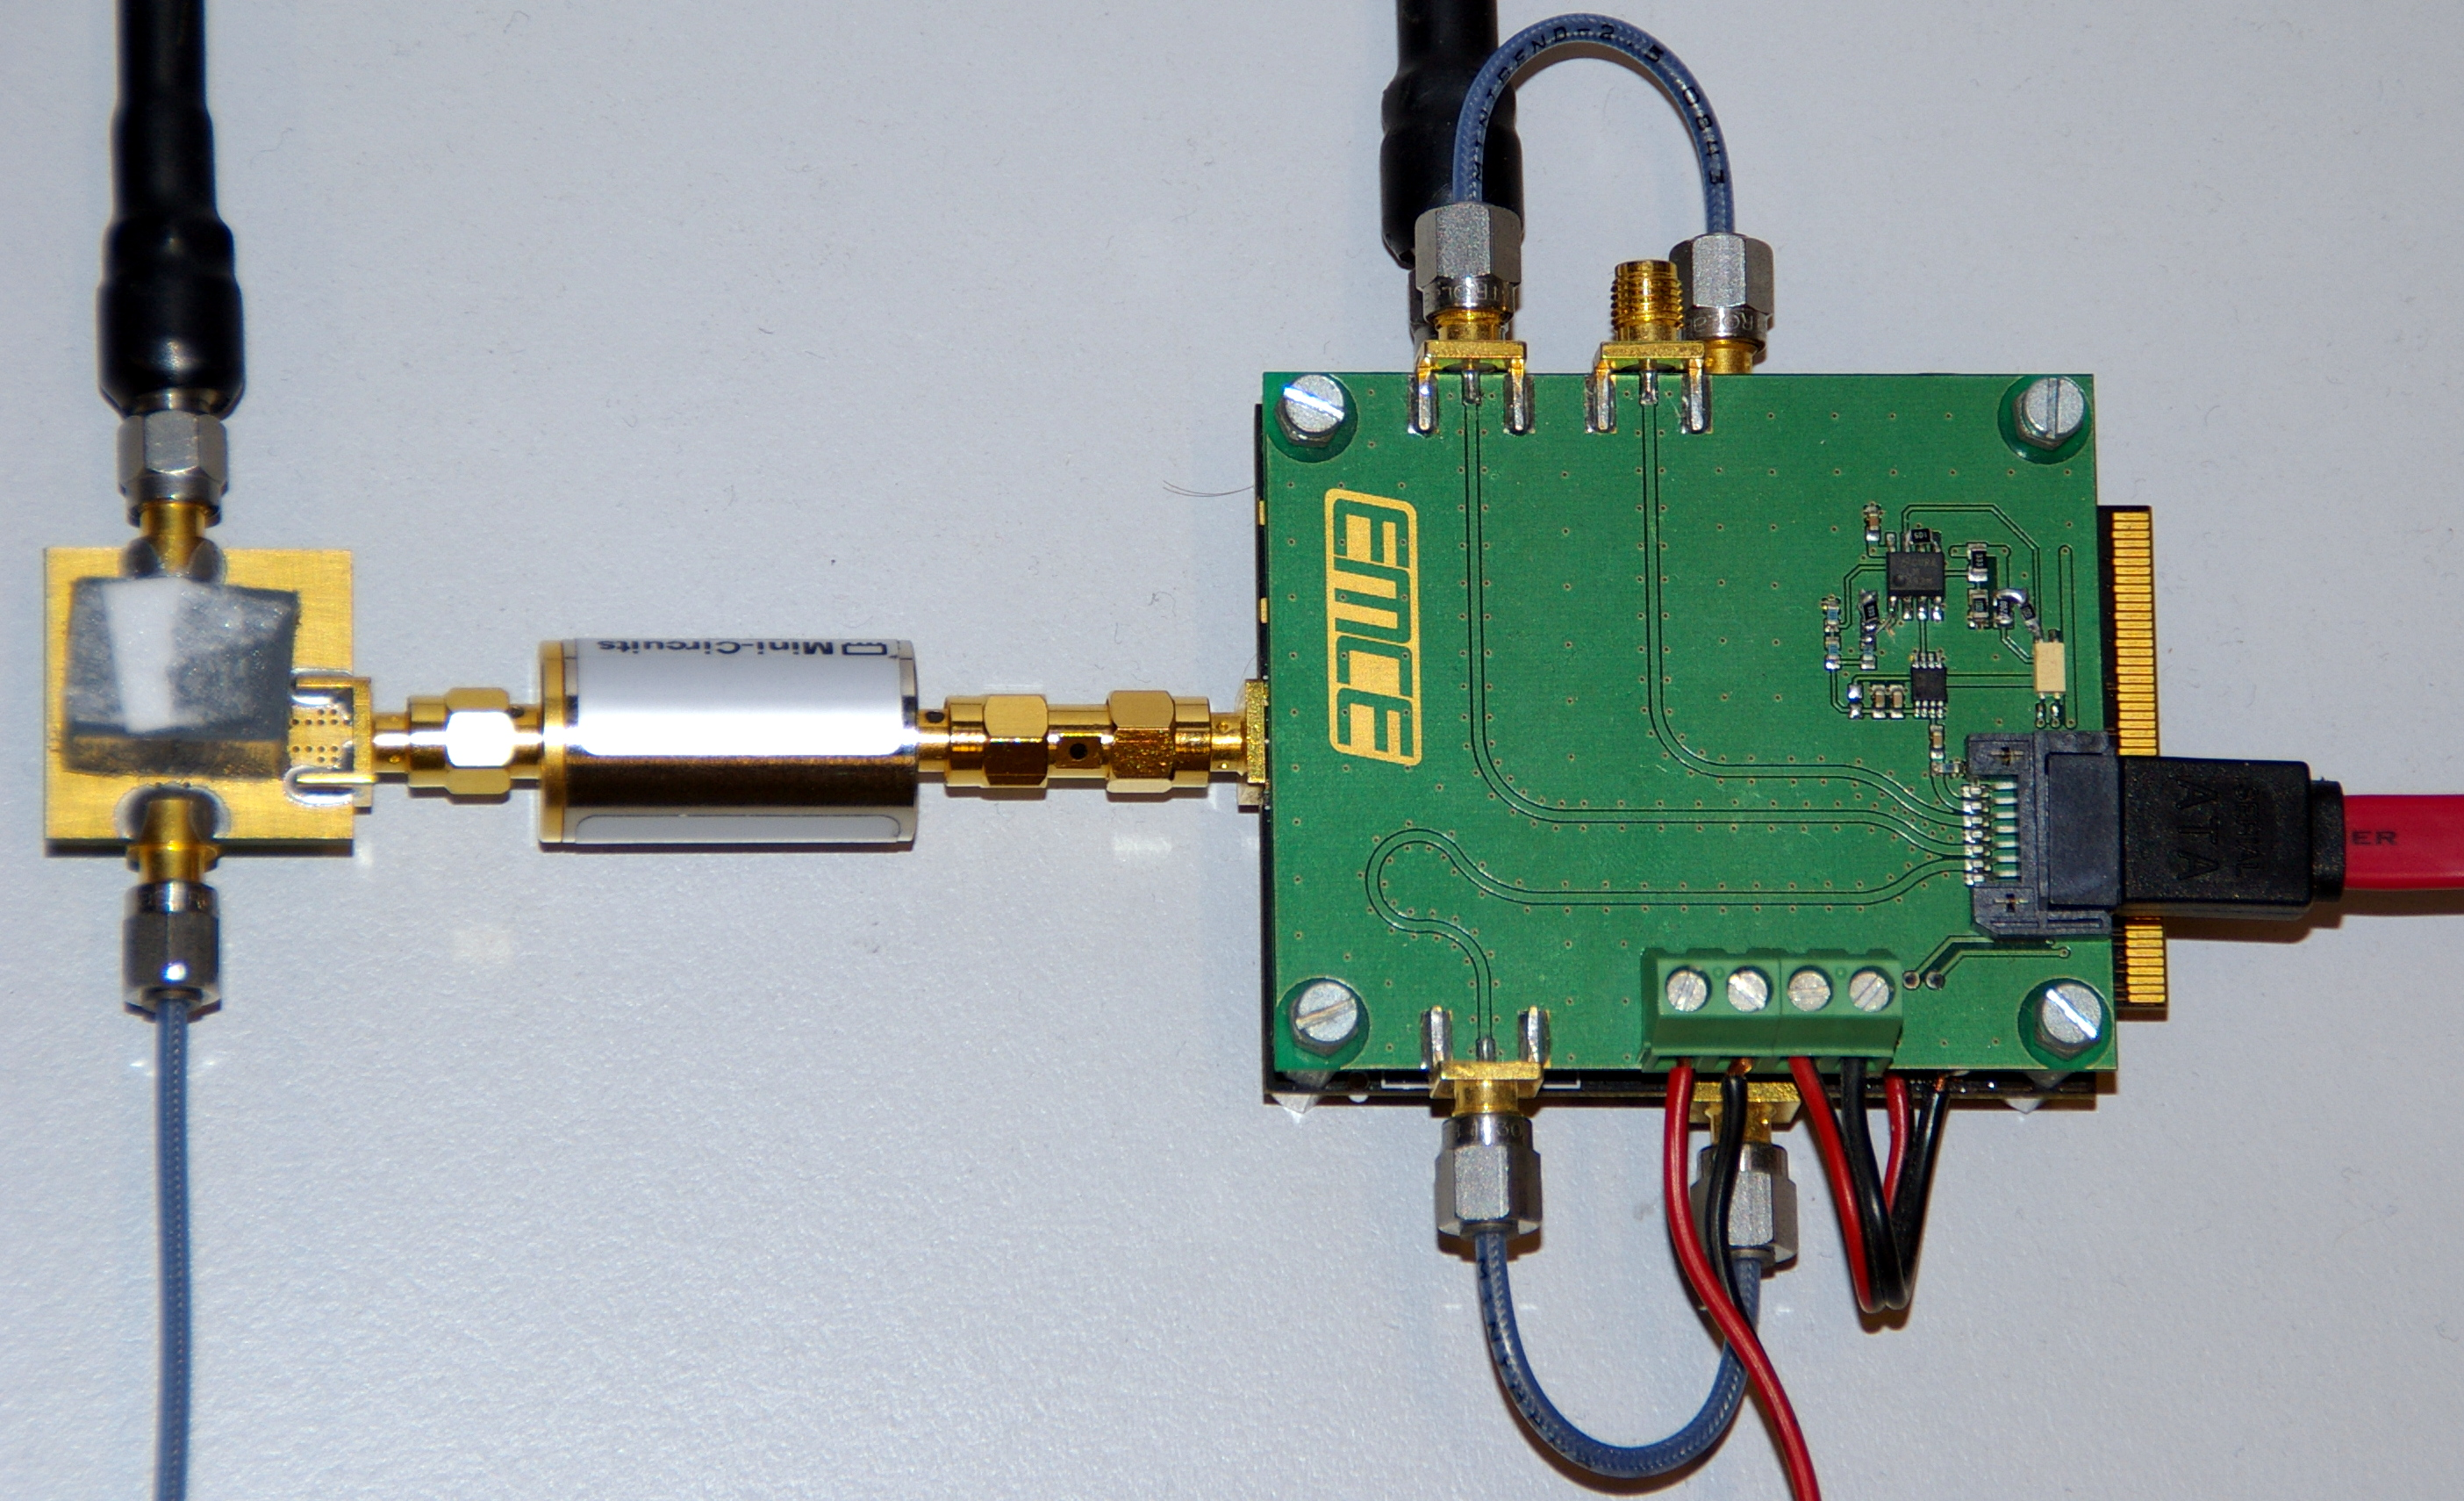
\includegraphics[width=4.5cm]{down_adc}
            \begin{itemize}
                \item Down conversion to \SI{70}{\mega\hertz} IF
                \item \SI{16}{\bit} \SI{100}{\mega\samples\per\second} ADC
                \item Bandpass sampling
            \end{itemize}
    \end{columns}
\end{frame}

\subsection{Digital Part}
\begin{frame}{Digital Part}
    \begin{columns}
        \column{5.5cm}
            \begin{tikzpicture}
                \pgfmathsetseed{23654}
                \tikzpicturedependsonfile{rfsymbols.tex}
                \draw node[coordinate,yshift=-1.5cm,label=left:$a_2$] (dac) {}

                      node[coordinate,yshift=1.5cm,label=left:$b_2$] (adc) {}
                      node[empty,right=of adc,label=below:buffer1] (inbuf) {}
                      node[mixer,right=of inbuf] (shift) {}
                      node[anchor=west] at (shift.east) {mix2}

                      (dac -| inbuf) node[mixer,label=above:mul1,generate] (mul) {}
                      node[empty,right=of mul] (outbuf) {}
                      node[anchor=north] at (outbuf.south) {buffer2}

                      ($(shift)!.5!(outbuf)$) node[allpass,generate] (H) {}
                      node[anchor=west] at (H.east) {fir1}

                      node[source,above=of shift.center,scale=0.7] (shiftsource) {}
                      node[anchor=east] at (shiftsource.west) {$\SI{30}{\mega\hertz}$}
                      node[anchor=west] at (shiftsource.east) {lo3}
                      node[below=of mul.center,fill=white] (gamma) {$\Gamma_{L,set}$};

                { [on background layer,every path/.style={dotted,decorate,decoration=random steps,segment length=2mm,thick}]
                    \draw ($(adc.east)!.5!(mul.west) + (0,4)$) -- ++(0,-7) node[coordinate] (rightsplit) {};
                }
                { [-latex,thick]
                    \draw[double] (shiftsource) -- (shift);
                    \draw[double,generate] (gamma) -- (mul);
                }
                { [latex-,dashed,every node/.style={font=\footnotesize},thick]
                    \foreach \device in {shiftsource} {
                        \draw (\device) -- ++(0,1) node[anchor=south] {ref};
                    }
                }
                { [start chain,every on chain/.style={join=by {-latex,incident,thick}}]
                    \chainin (adc);
                    \chainin (inbuf);
                    \chainin (shift);
                    { [every on chain/.style={join=by {double,-latex,incident,thick}}]
                        \chainin (H);
                        \chainin (outbuf);
                        \chainin (mul);
                    }
                }
                \draw[double,-latex,reflect,thick] (mul) -- (dac);
            \end{tikzpicture}
        \column{7cm}
            \begin{itemize}
                \item Down conversion to Baseband
                \item Fully configurable filter \device{fir1} implemented with circular convolution
                \item Multiplier for reflection synthesis
                \item \SI{16}{\bit} signal processing chain
                \item Implemented in FPGA
            \end{itemize}
            \hspace{1.5cm}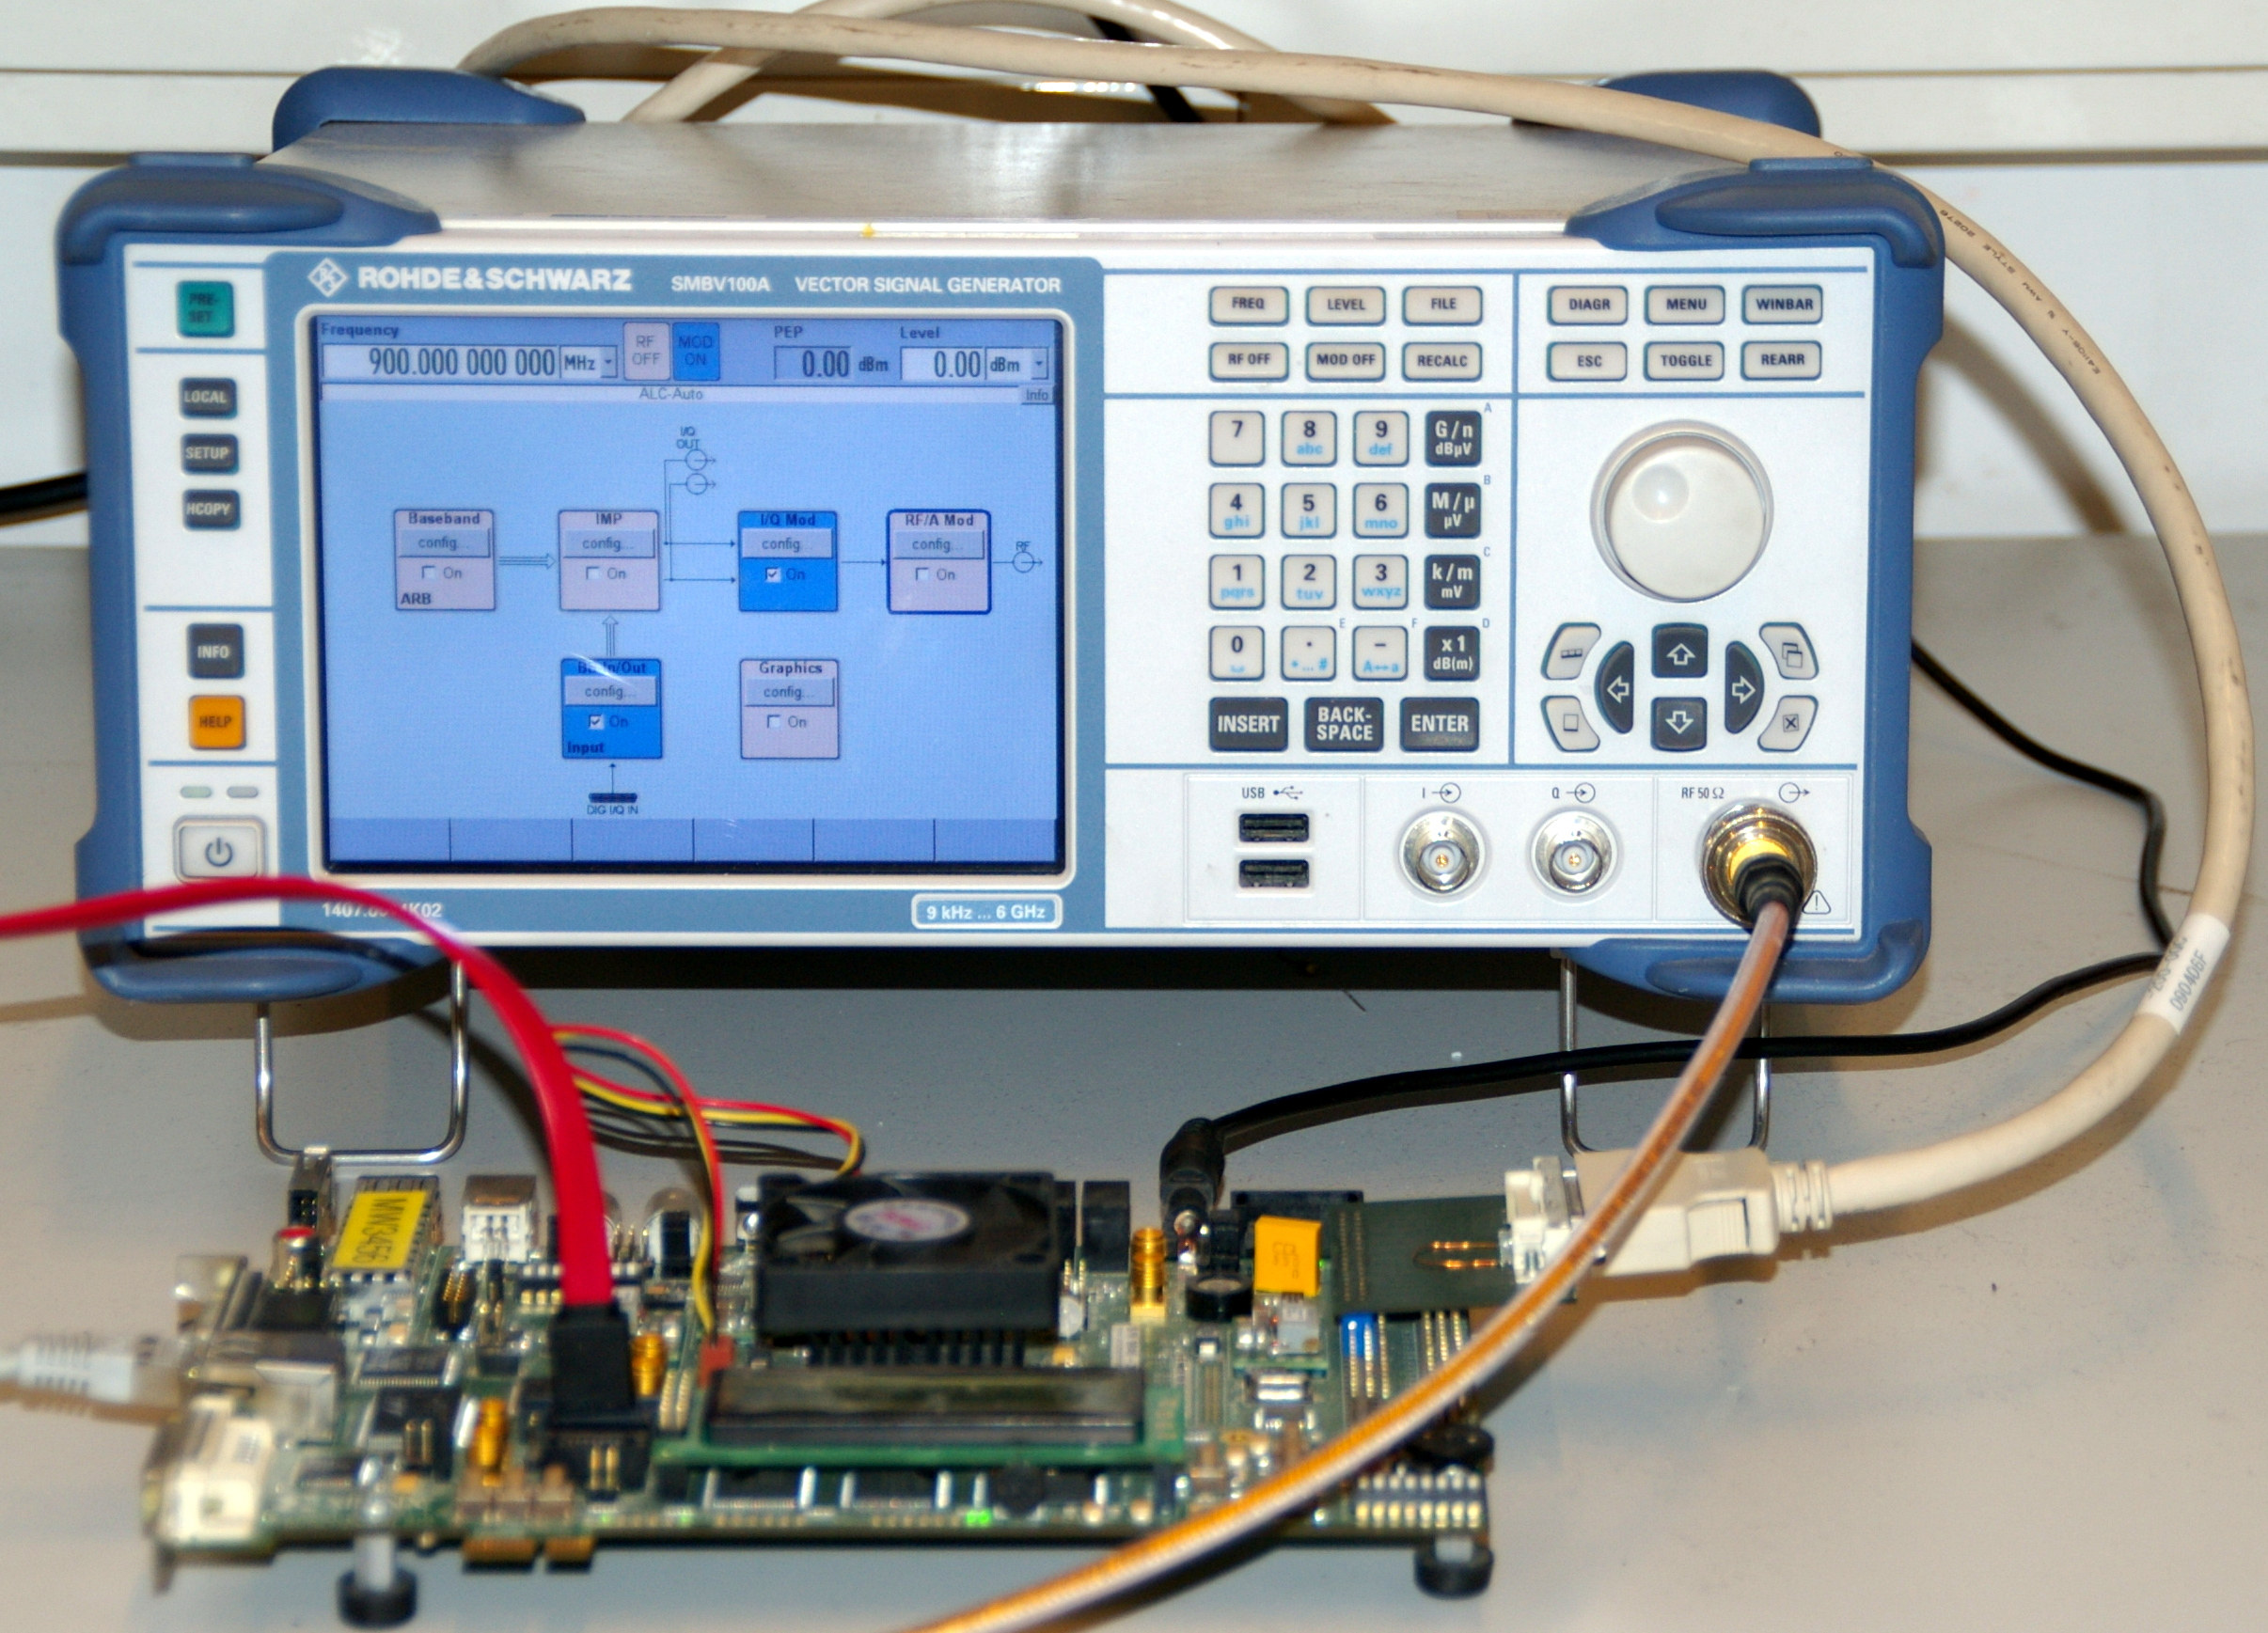
\includegraphics[width=5.5cm]{digital_part}
    \end{columns}
    \note{Buffers! Lag Time!}
\end{frame}

\section{Results}

\subsection{Reflection Synthesis}


\subsection{Filter performance}

\begin{frame}{Calibrated Filter, Uncalibrated $\Gamma_{L,set}$}
    \note{Uncalibrated $\Gamma_{L,set}$ (reflections from rest of setup!)}
    \note{\par Mean also possible}
    \begin{columns}
        \column{0.5\linewidth}
            \begin{tikzpicture}[every axis/.style={font=\tiny}]
                \begin{smithchart}[width=\linewidth,clip=false,title={\normalsize $0.5 \angle \SI{135}{\degree}$}]
                    \foreach \i in {1,...,11}{
                        \foreach \j in {1,...,11}{
                            \addplot[blue,is smithchart cs,line join=bevel] file {testdata/filter/0.5,135/\i,\j.data};
                        }
                    }
                    \addplot[red,is smithchart cs,mark=*,only marks] coordinates {(-0.3536,0.3536)};
                \end{smithchart}
            \end{tikzpicture}
        \column{0.5\linewidth}
            \begin{tikzpicture}[every axis/.style={font=\tiny}]
                \begin{smithchart}[width=\linewidth,clip=false,title={\normalsize $0.5 \angle \SI{-45}{\degree}$}]
                    \foreach \i in {1,...,11}{
                        \foreach \j in {1,...,11}{
                            \addplot[blue,is smithchart cs,line join=bevel] file {testdata/filter/0.5,-45/\i,\j.data};
                        }
                    }
                    \addplot[red,is smithchart cs,mark=*,only marks] coordinates {(0.3536,-0.3536)};
                \end{smithchart}
            \end{tikzpicture}
    \end{columns}
    \begin{center}
        11 by 11 grid $\Gamma_{L,set}$, \SI{11}{\mega\hertz} bandwidth
    \end{center}
\end{frame}

\section*{Summary}

\begin{frame}{Summary}
    \begin{block}{FPGA based load-pull System}
        \begin{itemize}
            \item Capable of synthesizing arbitrary $\Gamma_L$ (even \num{> 1})
        \end{itemize}
    \end{block}
    \begin{columns}
        \column{0.45\linewidth}
            \begin{block}{Iterative Target Algorithm}
                \begin{itemize}
                    \item Capable of setting $\Gamma_L$
                    \item Performance dependent on accuracy/time delay
                \end{itemize}
            \end{block}
        \column{0.45\linewidth}
            \begin{block}{Digital Filter}
                \begin{itemize}
                    \item Compensates frequency response
                    \item Ensures uniform $\Gamma_L$
                    \item Accurate in calibrated area
                \end{itemize}
            \end{block}
    \end{columns}
\end{frame}

% =============================================================================

\appendix
\backupbegin
\section<presentation>*{\appendixname}

\begin{frame}{System overview}
    \note[item]{One Port VNA}
    \note[item]{Analog}
    \note[item]{Digital}
    \note{\par Systematic Errors!! ($\Gamma_{L,set}$)}
    \resizebox{\linewidth}{!}{
    \begin{tikzpicture}
        \pgfdeclarelayer{foreground}
        \pgfsetlayers{background,main,foreground}
        \tikzpicturedependsonfile{rfsymbols.tex}
        \draw node[dut] (dut) {}
              node[dircoupler,right=2 of dut,label=below:dir1] (dirvna) {}
              node[oscilloscope,above=of dirvna.A2,anchor=A1] (oszivna) {}
              node[circulator,right=of dirvna,label=below:circ1] (circ) {}

              node[coordinate,right=of circ,yshift=1.5cm] (uppernode) {}
              node[coordinate,right=of circ,yshift=-1.5cm] (lowernode) {}

              (lowernode) node[amplifier,label=above:amp1] (amp) {}
              node[mixer,right=of amp,label=above:mix3] (upmix) {}
              node[lowpass,right=of upmix,label=above:lp1] (antialias) {}
              node[adc,right=of antialias,label=above:dac1] (dac) {}

              (uppernode -| upmix) node[mixer,label=below:mix1] (downmix) {}
              node[bandpass,right=of downmix,label=below:bp1] (bp) {}
              node[adc,right=of bp,label=below:adc1] (adc) {}
              node[empty,right=of adc,label=below:buffer1] (inbuf) {}
              node[mixer,right=of inbuf] (shift) {}
              node[anchor=west] at (shift.east) {mix2}

              (dac -| inbuf) node[mixer,label=above:mul1,generate] (mul) {}
              node[empty,right=of mul] (outbuf) {}
              node[anchor=north] at (outbuf.south) {buffer2}

              ($(shift)!.5!(outbuf)$) node[allpass,generate] (H) {}
              node[anchor=west] at (H.east) {fir1}

              node[source,above=of downmix.center,scale=0.7] (downsource) {}
              node[anchor=west] at (downsource.east) {lo1}
              node[source,above=of adc.center,scale=0.7] (sample) {}
              node[anchor=west] at (sample.east) {lo2}
              node[source,above=of shift.center,scale=0.7] (shiftsource) {}
              node[anchor=west] at (shiftsource.east) {lo3}
              node[source,below=of upmix.center,scale=0.7] (upsource) {}
              node[anchor=west] at (upsource.east) {lo4}
              node[below=of mul.center] (gamma) {$\Gamma_{L,set}$};

        \draw ($(dut)!.5!(dirvna)$) node[coordinate] (plane) {};

        { [rounded corners=2pt,thick]
            \draw (dut) -- (dirvna) -- (circ.A);
            \draw[incident] [-latex] (circ.B) -- ($(circ.B |- uppernode)!.5!(uppernode)$) node[coordinate] (upper) {} -- (downmix);
            \draw[incident] (dirvna.A2) -- (oszivna.A1);
            \draw[reflect] (dirvna.B2) |- ($(dirvna.B2)!.7!(oszivna.A2)$) node[coordinate] (oszimiddle) {} -| (oszivna.A2);
            \draw[reflect] [-latex] (amp) -- ($(circ.C |- amp)!.5!(lowernode)$) node[coordinate] (lower) {} -- (circ.C);
        }
        { [-latex,thick]
            \draw (downsource) -- (downmix);
            \draw (sample) -- (adc);
            \draw [double] (shiftsource) -- (shift);
            \draw[generate,double] (gamma) -- (mul);
            \draw (upsource) -- (upmix);
        }
        { [latex-,dashed,every node/.style={font=\footnotesize},thick]
            \foreach \device in {downsource,sample,shiftsource} {
                \draw (\device) -- ++(0,1) node[anchor=south] {ref};
            }
            \draw ([xshift=0.5cm]oszivna.north) -- ++(0,0.5) node[fill=white,anchor=south] {ref};
            \draw (upsource) -- ++(0,-1) node[anchor=north] {ref};
        }
        { [start chain,every on chain/.style={join=by {-latex,incident,thick}}]
            \chainin (downmix);
            \chainin (bp);
            \chainin (adc);
            \chainin (inbuf);
            \chainin (shift);
            { [every on chain/.style={join=by {double,-latex,incident,thick}}]
                \chainin (H);
                \chainin (outbuf);
                \chainin (mul);
            }
        }
        { [start chain,every on chain/.style={join=by {-latex,reflect,thick}}]
            { [every on chain/.style={join=by {double,-latex,reflect,thick}}]
                \chainin (mul);
                \chainin (dac);
                \chainin (antialias);
                \chainin (upmix);
            }
            \chainin (amp);
        }
        { [on background layer,every path/.style={dotted,decorate,decoration=random steps,segment length=2mm,thick}]
            \draw ($(dirvna.B1)!.5!(circ.A) + (0,4)$) -- ++(0,-8.5) node[coordinate] (leftsplit) {};
            \draw ($(adc.east)!.5!(mul.west) + (0,4)$) -- ++(0,-8.5) node[coordinate] (rightsplit) {};
        }

        \draw (leftsplit) node[anchor=base east] {One Port VNA}
              (leftsplit) node[anchor=base west] {Analog}
              (rightsplit) node[anchor=base west] {Digital}
              (rightsplit) node[anchor=base east] {Analog};

        \draw [dashed] ($(plane) + (0,4)$) node[anchor=south] {Load Reference Plane} -- ($(plane) - (0,4.5)$);

        \draw [latex-] ($(plane) + (0,1.5)$) -- ++(-0.5,0) node[anchor=east] {$Z_L$};

        \draw [-latex,reflect] ($(plane) + (0.25,-1.5)$) node[anchor=west] {$a_2$}-- ++(-0.5,0);
        \draw [latex-,incident] ($(plane) + (0.25,-2)$) node[anchor=west] {$b_2$}-- ++(-0.5,0);
        \draw [latex-] ($(plane) + (0,-2.5)$) -- ++(-0.5,0) node[anchor=east] {$\Gamma_L$};

        {[densely dashdotdotted,latex-latex,thick]
            \draw ($(inbuf.north) + (0,1)$) -- ++(0,1) node [anchor=south] {PC};
            \draw ([xshift=-0.5cm]oszivna.north) -- ++(0,1) node [anchor=south] {PC};
        }
    \end{tikzpicture}
    }
\end{frame}

\begin{frame}
    \begin{columns}
        \note{$a$ $b$: DFT}
        \column{5cm}
            \tikzset{external/export next=false}
            \begin{tikzpicture}
                \pgfmathsetseed{23654}
                \pgfdeclarelayer{foreground}
                \pgfsetlayers{background,main,foreground}
                \tikzpicturedependsonfile{rfsymbols.tex}
                \tikzstyle{every node}=[font=\footnotesize]
                \draw node[dut] (dut) {}
                      node[dircoupler,right=2 of dut,label=below:dir1] (dirvna) {}
                      node[oscilloscope,above=of dirvna.A2,anchor=A1] (oszivna) {}
                      node[coordinate,right=1.5em of dirvna] (rest) {}
                      node[coordinate,right=1.5em of rest] (resta) {};

                \draw ($(dut)!.5!(dirvna)$) node[coordinate] (plane) {};

                \draw [dashed] (rest) -- (resta);

                { [rounded corners=2pt]
                    \draw (dut) -- (dirvna) -- (rest);
                    \draw[incident] (dirvna.A2) -- (oszivna.A1);
                    \draw[reflect] (dirvna.B2) |- ($(dirvna.B2)!.7!(oszivna.A2)$) node[coordinate] (oszimiddle) {} -| (oszivna.A2);
                }
                { [latex-,dashed,every node/.style={font=\footnotesize}]
                    \draw ([xshift=0.5cm]oszivna.north) -- ++(0,0.5) node[fill=white,anchor=south] {ref};
                }
                { [on background layer,every path/.style={dotted,decorate,decoration=random steps,segment length=2mm,thick}]
                    \draw ($(rest) + (0,4)$) -- ++(0,-7) node[coordinate] (leftsplit) {};
                }

                \draw (leftsplit) node[anchor=base east] {One Port VNA}
                      (leftsplit) node[anchor=base west] {Analog};

                \draw [-latex,incident] ($(dirvna.A2) + (-0.2,0.1)$) -- node[base left] {$b'_2$} ($(oszivna.A1 |- oszimiddle) - (0.2,0.1)$);
                \begin{pgfonlayer}{foreground}
                    \draw [-latex,reflect] ($(dirvna.B2) + (0.2,0.1)$) -- node[coordinate] (a1) {} ($(oszimiddle -| dirvna.B2) + (0.2,-0.1)$);
                \end{pgfonlayer}
                \draw (a1) node[base right,reflect] {$a'_2$};

                \draw [dashed] ($(plane) + (0,4)$) node[anchor=south] {Load Reference Plane} -- ($(plane) - (0,3)$);

                \draw [latex-] ($(plane) + (0,1.5)$) -- ++(-0.5,0) node[anchor=east] {$Z_L$};

                \draw [-latex,reflect] ($(plane) + (0.25,-1.5)$) node[anchor=west] {$a_2$}-- ++(-0.5,0);
                \draw [latex-,incident] ($(plane) + (0.25,-2)$) node[anchor=west] {$b_2$}-- ++(-0.5,0);
                \draw [latex-] ($(plane) + (0,-2.5)$) -- ++(-0.5,0) node[anchor=east] {$\Gamma_L$};

                {[densely dashdotdotted,latex-latex]
                    \draw ([xshift=-0.5cm]oszivna.north) -- ++(0,1) node [anchor=south] {PC};
                }
            \end{tikzpicture}
        \column{5cm}
            \begin{enumerate}
                \item Acquire \textcolor{incident}{$a_1$}, \textcolor{reflect}{$b_1$}
                \item Extract phase and magnitude
                \tikzset{external/export next=false}
                \item $\Gamma_L = \frac{\textcolor{reflect}{a_2}}{\textcolor{incident}{b_2}} \tikz[remember picture,baseline] \node[anchor=base] (approx) {$\approx$}; \frac{\textcolor{reflect}{a'_2}}{\textcolor{incident}{b'_2}}$
                    \tikzset{external/export next=false}
                    \tikz[overlay,remember picture] \draw [latex-] (approx.south) -- ++(0,-2em) node[below] {Systematic Errors};
            \end{enumerate}
    \end{columns}
\end{frame}

\begin{frame}{Errorbox One Port VNA}
    \begin{columns}
        \column{5cm}
            \begin{tikzpicture}
                \matrix (box)
                [matrix of nodes,%
                 nodes in empty cells,
                 nodes={dspnodeopen},
                 column sep=0.5cm,
                 row sep=2cm,
                 ampersand replacement=\&]
                {
                    |[coordinate]| \& \&[3cm] \& \&[.5cm] |[coordinate]| \\
                    |[coordinate]| \& \& \& \& |[coordinate]| \\
                };
                \draw[-latex] (box-1-1) node[anchor=east] {$a_{1}$} -- (box-1-2);
                \draw[-latex] (box-1-2) -- node[above] {$1$} (box-1-3);
                \draw[-latex] (box-1-3) -- node[above] {$b_{2}$} (box-1-4);

                \draw[latex-] (box-2-1) node[anchor=east] {$b_{1}$} -- (box-2-2);
                \draw[latex-] (box-2-2) -- node[above] {$S_{12}$} (box-2-3);
                \draw[latex-] (box-2-3) -- node[above] {$a_{2}$} (box-2-4);

                \draw[-latex] (box-1-2) to[bend left=30] node[right] {$S_{11}$} (box-2-2);
                \draw[latex-] (box-1-3) to[bend right=30] node[left] {$S_{22}$} (box-2-3);

                \draw[-latex] (box-1-4) to[bend left=30] node[right] {$\Gamma_L$} (box-2-4);

                \draw ($(box-1-2) + (0,0.7cm)$) rectangle ($(box-2-3) - (0,0.7cm)$);
                \draw ($(box-1-4) + (0,0.7cm)$) rectangle ($(box-2-5) - (0,0.7cm)$);

                \draw[dashed] (box-1-2) -- ++(0,1.5cm) node[anchor=south] {Oscilloscope};
                \draw[dashed] (box-1-3) -- ++(0,1.5cm) node[anchor=south] {Load Reference Plane};

                \draw[dashed] (box-2-2) -- ++(0,-1cm);
                \draw[dashed] (box-2-3) -- ++(0,-1cm);

                \draw ($(box-2-4)!.5!(box-2-5) - (0,0.7cm)$) node[anchor=north] {DUT};
                \draw ($(box-2-2)!.5!(box-2-3) - (0,0.7cm)$) node[anchor=north] {Error box};
            \end{tikzpicture}
        \column{5cm}
            \begin{description}
                \item[$S_{11}$] Directivity
                \note[item]{Directivity: Reflections not from DUT}
                \item[$S_{12}$] Reflection tracking
                \note[item]{Reflection Tracking: Frequency response oscilloscope ports; coupler loss; transmission lines}
                \item[$S_{22}$] Source match
                \note[item]{Source match: Mismatch DUT/Measurement system}
            \end{description}
    \end{columns}
\end{frame}

\begin{frame}{Iterative Target Algorithm}
    \begin{enumerate}
        \item Arbitrary start point
        \item Measure $\Gamma_L$
        \item If $\abs{\Gamma_L - \Gamma_{L,target}} < accuracy$ \Rightarrow done
        \item Scale $\Gamma_{L,set}$ according to $\frac{\Gamma_{L,target}}{\Gamma_L}$
        \item Pause to compensate for lag time
        \item Repeat from step 2
    \end{enumerate}
\end{frame}

\begin{frame}[fragile]{Target algorithm 1}
    \note{Good}
    \begin{columns}
        \column{9cm}
            \tikzset{external/export next=false}
            \begin{tikzpicture}[
                spy/.style={%
                    draw,green,
                    line width=0.5pt,
                    circle,inner sep=0pt,
                },
                every axis/.style={font=\footnotesize},
                ]
                \def\spyviewersize{3cm}
                \def\spyonclipreduce{0.5pt}
                \def\spyfactorI{10}

                \def\pic#1#2{
                    \begin{smithchart}[width=7cm,clip=false#1]
                        \addplot[blue,is smithchart cs,line join=bevel] file {testdata/filter/1.0,0/trajectory10.data};
                        \addplot[purple,is smithchart cs,only marks,mark=x#2] file {testdata/filter/1.0,0/trajectory10.data};
                        \draw (cartesian cs:1,0) node[coordinate] (a) {}
                              (cartesian cs:-0.4,0.4) node[coordinate] (b) {};
                    \end{smithchart}
                }
                \pic{}{}
                \coordinate (spy-on 1) at (a);
                \coordinate (spy-in 1) at (b);

                \node[spy,ultra thick,circular drop shadow,minimum size=\spyviewersize,fill=white,label={[inner sep=2pt,yshift=-5pt,fill=white,font=\small]below:\spyfactorI{}x magnification}] (spy-in node 1) at (spy-in 1) {};
                \begin{scope}
                    \clip (spy-in 1) circle (0.5*\spyviewersize-\spyonclipreduce);
                    \pgfmathsetmacro\sI{1/\spyfactorI}
                    \begin{scope}[
                        shift={($\sI*(spy-in 1)-\sI*(spy-on 1)$)},
                        scale around={\spyfactorI:(spy-on 1)}
                    ]
                    \pic{,every axis plot post/.append style={line width=0.07pt},every axis/.append style={line width=0.07pt,grid style={line width=0.07pt}}}{,mark size=0.35pt}
                    \end{scope}
                \end{scope}

            \end{tikzpicture}
        \column{4cm}
            $\Gamma_{L,target} = 1$
    \end{columns}
\end{frame}

\begin{frame}[fragile]{Target algorithm 2}
    \note{Bad! Target area accuracy}
    \begin{columns}
        \column{9cm}
            \tikzset{external/export next=false}
            \begin{tikzpicture}[
                spy/.style={%
                    draw,green,
                    line width=0.5pt,
                    circle,inner sep=0pt,
                },
                every axis/.style={font=\footnotesize},
                ]
                \def\spyviewersize{3cm}
                \def\spyonclipreduce{0.5pt}
                \def\spyfactorI{50}

                \def\pic#1#2{
                    \begin{smithchart}[width=7cm,clip=false#1]
                        \addplot[blue,is smithchart cs,line join=bevel] file {testdata/filter/0.5,-45/trajectory6.data};
                        \addplot[purple,is smithchart cs,only marks,mark=x#2] file {testdata/filter/0.5,-45/trajectory6.data};
                        \draw (cartesian cs:0.35325,-0.35397) node[coordinate] (a) {}
                              (cartesian cs:-0.4,0.4) node[coordinate] (b) {};
                    \end{smithchart}
                }
                \pic{}{}
                \coordinate (spy-on 1) at (a);
                \coordinate (spy-in 1) at (b);

                \node[spy,ultra thick,circular drop shadow,minimum size=\spyviewersize,fill=white,label={[inner sep=2pt,yshift=-5pt,fill=white,font=\small]below:\spyfactorI{}x magnification}] (spy-in node 1) at (spy-in 1) {};
                \begin{scope}
                    \clip (spy-in 1) circle (0.5*\spyviewersize-\spyonclipreduce);
                    \pgfmathsetmacro\sI{1/\spyfactorI}
                    \begin{scope}[
                        shift={($\sI*(spy-in 1)-\sI*(spy-on 1)$)},
                        scale around={\spyfactorI:(spy-on 1)}
                    ]
                        \pic{,every axis plot post/.append style={line width=0.01pt}}{,mark size=0.06pt}
                    \end{scope}
                \end{scope}
            \end{tikzpicture}
        \column{4cm}
            $\Gamma_{L,target} = 0.5 \angle \SI{-45}{\degree}$
    \end{columns}
\end{frame}

\begin{frame}{Target algorithm performance}
    \note{Previous only one in bin 8}
    \begin{columns}
        \column{7cm}
            \begin{tikzpicture}
                \begin{axis}[
                        title = 108 algorithm invocations,
                        ybar interval,
                        ylabel={percentage of invocations},
                        xlabel={number of iterations},
                        x filter/.expression={x-1}, % remove the start point
                        width=7cm,
                        ymin = 0
                    ]
                    \addplot[blue,fill=blue!10,hist={bins=7,data min=3,data max=10,density=true}] table[y index=0] {testdata/trajectories/performance.data};
                \end{axis}
            \end{tikzpicture}
        \column{5cm}
            \begin{block}{Performance dependent on}
                \begin{itemize}
                    \item Start point
                    \item Target
                    \item Resolution in target area
                    \item Pause for lag time compensation
                \end{itemize}
            \end{block}
    \end{columns}
\end{frame}

        \def\bpspec#1#2{%
            \begin{scope}[shift={#1}]
                \draw [#2] (-0.2,0) -- (-0.2,0.5) -- (0.2,0.8) -- (0.2,0);
            \end{scope}
        }

\begin{frame}{Down Conversion Spectra}
    \resizebox{\linewidth}{!}{
    \begin{tikzpicture}[every node/.style={font=\small},every path/.style={decoration={name=zigzag,segment length=2pt}}]
        \begin{scope}[shift={(0,6)}]
            \draw [latex-latex] (-5,0) -- (3,0) decorate { -- (3.1,0) } -- (5,0) node[anchor= west] {frequency};
            \draw [-latex] (0,-0.2) -- (0,1) node[anchor=south] {amplitude};
            \bpspec{(3.5,0)}{solid,thick}
            \draw (3.5,0.1) -- (3.5,-0.1) node[anchor=north] {$f_0$};
            \draw (-5,0.5) node[anchor=east,font={}] (rf) {RF};
            \draw [-latex] (3.5,0) to[bend left=30] ($0.7*(2,0)$);
            \draw ($0.7*(2,0) + (0,0.1)$) -- ($0.7*(2,0) - (0,0.1)$) node[anchor=north] {$\SI{70}{\mega\hertz}$};
        \end{scope}
        \begin{scope}[shift={(0,4)}]
            \draw [latex-latex] (-5,0) -- (4,0) decorate { -- (4.1,0) } -- (5,0) node[anchor=west] {frequency};
            \draw [-latex] (0,-0.2) -- (0,1);
            \bpspec{(4.5,0)}{dashed}
            \draw (4.5,0.1) -- (4.5,-0.1) node[anchor=north] {$2f_0 + \SI{70}{\mega\hertz}$};
            \bpspec{($0.7*(2,0)$)}{solid,thick}
            \draw ($0.7*(2,0) + (0,0.1)$) -- ($0.7*(2,0) - (0,0.1)$) node[anchor=north] {$\SI{70}{\mega\hertz}$};
            \draw (-5,0.5) node[anchor=east,font={}] (if) {IF};
            \draw [dashed,very thick,-latex] (0,0) -- (0,0.8);
        \end{scope}
        \begin{scope}[shift={(0,2)}]
            \draw [latex-latex] (-5,0) -- (5,0) node[anchor=west] {frequency};
            \draw [-latex] (0,-0.2) -- (0,1);
            \foreach \x in {-2,-1,1,2} {
                \draw ($\x*(2,0) + (0,0.1)$) -- ($\x*(2,0) - (0,0.1)$) node[anchor=north] {$\x f_s$};
                \draw [dotted] ($\x*(2,0)$) -- ($\x*(2,0) + (0,1)$);
                \draw [thick,-latex,dashed] ($\x*(2,0)$) -- ($\x*(2,0) + (0,0.8)$);
            }
            \foreach \x in {-3,-2,0,1} {
                \bpspec{($0.7*(2,0) + \x*(2,0)$)}{dashed}
            }
            \begin{scope}[xscale=-1]
                \foreach \x in {-3,...,1} {
                    \bpspec{($0.7*(2,0) + \x*(2,0)$)}{dashed}
                }
            \end{scope}
            \bpspec{($0.7*(2,0) + -1*(2,0)$)}{solid,thick}
            \draw [-latex] ($0.7*(2,0) - (2,0)$) to[bend right=45] (0,0);
            \draw ($0.7*(2,0) + -1*(2,0) + (0,0.1)$) -- ($0.7*(2,0) + -1*(2,0) + (0,-0.1)$) node[anchor=north] {$\SI{-30}{\mega\hertz}$};
            \draw (-5,0.5) node[anchor=east,font={}] (sample) {sampling};
            \draw [very thick,-latex,dashed] (0,0) -- (0,0.8);
        \end{scope}
        \draw [latex-latex] (-5,0) -- (5,0) node[anchor=west] {frequency};
        \draw [-latex] (0,-0.2) -- (0,1);
        \foreach \x in {-2,-1,1,2} {
            \draw ($\x*(2,0) + (0,0.1)$) -- ($\x*(2,0) - (0,0.1)$) node[anchor=north] {$\x f_s$};
            \draw [dotted] ($\x*(2,0)$) -- ($\x*(2,0) + (0,1)$);
        }
        \bpspec{(0,0)}{solid,thick}
        \draw (-5,0.5) node[anchor=east,font={}] (mix) {digital mixer};
        \draw [-latex] ([xshift=-5pt]rf.south east) -- ([xshift=-5pt]if.north east);
        \draw [-latex] ([xshift=-5pt]if.south east) -- ([xshift=-5pt]sample.north east);
        \draw [-latex] ([xshift=-5pt]sample.south east) -- ([xshift=-5pt]mix.north east);
        \foreach \x in {-3,-2,0,1} {
            \bpspec{($(2,0) + \x*(2,0)$)}{dashed}
        }
        \begin{scope}[xscale=-1]
            \foreach \x in {-2,...,2} {
                \bpspec{($0.4*(2,0) + \x*(2,0)$)}{dashed}
            }
        \end{scope}
        \foreach \x in {-2,...,2} {
            \draw [thick,-latex,dashed] ($\x*(2,0) + 0.3*(2,0)$) -- ($\x*(2,0) + 0.3*(2,0) + (0,0.8)$);
        }
    \end{tikzpicture}
    }
\end{frame}

\begin{frame}{Overlap Add Algorithm}
\begin{figure}[htb]
    \centering
    \begin{tikzpicture}
        \begin{scope}[shift={(0,13em)}]
            \draw [decorate,decoration={brace},yshift=2pt] (0,4.1em) -- (5,4.1em) node[midway,yshift=8pt] {$n$};
            \draw [decorate,decoration={brace},yshift=2pt] (0,2.8em) -- (3,2.8em) node[midway,yshift=8pt] {$n_{fft}$};
            \draw [decorate,decoration={brace},yshift=2pt] (0,1.5em) -- (2,1.5em) node[midway,yshift=8pt] {$L$};
            \draw (0,0.75em) node[anchor=east] {$x[n]$};
            \draw (0,0) rectangle (5,1.5em);
            \draw (5,0.75em) node[anchor=west] (zeros) {0000};
            \draw [dashed] (5,0) rectangle (6,1.5em) (2,0) -- (2,1.5em) (4,0) -- (4,1.5em);
        \end{scope}
        \begin{scope}[shift={(0,9em)}]
            \draw (0,0.75em) node[anchor=east] {$y_0[n]$};
            \draw (0,0) rectangle (2,1.5em);
            \draw [fill=black!30] (2,0) rectangle (3,1.5em);
            \draw (2.5,0) node[coordinate] (y0b) {};
            \draw (0.5,0) node[coordinate] (y2b) {};
        \end{scope}
        \begin{scope}[shift={(0,6em)}]
            \draw (0,0.75em) node[anchor=east] {$y_1[n]$};
            \draw (2,0) rectangle (4,1.5em);
            \draw [fill=black!30] (4,0) rectangle (5,1.5em);
            \draw (2.5,1.5em) node[coordinate] (y1t) {};
            \draw (4.5,0) node[coordinate] (y1b) {};
        \end{scope}
        \begin{scope}[shift={(0,3em)}]
            \draw (0,0.75em) node[anchor=east] {$y_2[n]$};
            \draw (4,0) rectangle (6,1.5em);
            \draw [fill=black!30] (6,0) rectangle (7,1.5em);
            \draw [fill=red!30] (0,0) rectangle (1,1.5em);
            \draw (1,0.75em) node[coordinate] (circto) {};
            \draw (4.5,1.5em) node[coordinate] (y2t) {};
            \draw (0.5,1.5em) node[coordinate] (ynt) {};
        \end{scope}
        \draw (0,0.75em) node[anchor=east] {$y[n]$};
        \draw (0,0) rectangle (5,1.5em);
        \draw [dashed,color=red] (5,0) rectangle (6,1.5em);
        \draw [dotted] (6,1.5em) rectangle (7,0em);
        \draw [latex-,color=red] (circto) parabola (5.5,1.5em);

        \draw ($(y0b)!.5!(y1t)$) node {$+$};
        \draw ($(y1b)!.5!(y2t)$) node {$+$};
        \draw ($(y2b)!.5!(ynt)$) node {$+$};
        \draw [dotted]
              (0,1.5em) -- (0,13em)
              (1,1.5em) -- (1,9em)
              (2,1.5em) -- (2,9em)
              (3,7.5em) -- (3,9em)
              (3,1.5em) -- (3,6em)
              (4,1.5em) -- (4,6em)
              (5,1.5em) -- (5,3em)
              (5,4.5em) -- (5,6em)
              (7,1.5em) -- (7,3em)
              (2,13em) -- (3,10.5em)
              (4,13em) -- (5,10.5em) -- (5,7.5em)
              (6,13em) -- (7,10.5em) -- (7,4.5em);
    \end{tikzpicture}
\end{figure}
\end{frame}

\begin{frame}{FPGA Design}
    \resizebox{\linewidth}{!}{
    \begin{tikzpicture}[every node/.style={minimum width=5em},latex-latex]
        \matrix (peripherals)[matrix of nodes,column sep=1em,row sep=0.2em,nodes={draw,anchor=center},ampersand replacement=\&]
        {
            DRAM \& \shortstack{DRAM\\Controller} \\
            Ethernet \& \shortstack{Ethernet\\Controller} \\
            RS232 \& \shortstack{RS232\\Interface} \\
            Storage \& SysAce \\
            \shortstack{LEDS\\Switches} \& GPIO \\
        };
        \node[draw,minimum size=5em,above right=0em of peripherals] (cpu) {CPU};
        \draw (peripherals-1-1) -- (peripherals-1-2);
        \draw (peripherals-1-2) -| ([xshift=-2.5em]cpu);
        \draw ([yshift=1em]peripherals-2-2) -| ([xshift=-1.5em]cpu);
        \foreach \i in {2,...,5}
        {
            \draw (peripherals-\i-1) -- (peripherals-\i-2);
            \draw (peripherals-\i-2) -- (peripherals-\i-2 -| cpu);
        }
        \draw[ultra thick,-] (peripherals-5-2 -| cpu) ++(0,-1em) node[below] (plb) {PLB} -- (cpu);
        \node[draw] at ($(peripherals-5-2)!2!(peripherals-5-2 -| cpu)$) (bram) {RAM};
        \draw (peripherals-5-2 -| cpu) -- (bram);
        \node[draw] at ($(peripherals-2-2)!2!(peripherals-2-2 -| cpu)$) (pint) {\shortstack{Processor\\Interface}};
        \draw (peripherals-2-2 -| cpu) -- (pint);
        \matrix (internal)[matrix of nodes,column sep=1em,row sep=0.2em,nodes={draw,anchor=center},right=of pint]
        {
            inbuf \\
            core \\
            outbuf \\
            auto \\
        };
        \node[draw,right=1.5em of internal-3-1] (digiq) {Digital I/Q};
        \node[draw,right=1.5em of internal-1-1] (adc) {ADC};
        \node[coordinate] at ($(pint.east) + (2em,0)$) (l) {};
        \foreach \i in {1,...,4}
        {
            \draw (pint.east) -- (l) |- (internal-\i-1);
        };
        \draw (internal-1-1) -- (adc);
        \draw (internal-3-1) -- (digiq);
        \node[draw,fit=(internal-1-1) (internal-4-1) (l),inner xsep=0.5em,label=main] (main) {};
        \node[draw,fit=(cpu) (peripherals-5-2) (plb) (main),inner xsep=0.5em,label=top] (fpga) {};

    \end{tikzpicture}
    }
\end{frame}

\begin{frame}{Architecture}
    \resizebox{\linewidth}{!}{
    \begin{tikzpicture}
        \tikzset{module/.style={fill=Pastel1-8-1}}
        \tikzset{interface/.style={fill=Pastel1-8-2}}
        \tikzset{cpu/.style={fill=Pastel1-8-3}}
        \tikzset{kernel/.style={fill=Pastel1-8-4}}
        \tikzset{software/.style={fill=Pastel1-8-5}}
        \tikzset{digital/.style={fill=Pastel1-8-6}}
        \tikzset{pc/.style={fill=Pastel1-8-7}}
        \tikzset{os/.style={fill=Pastel1-8-8}}

        \node[anchor=base west,inner xsep=.5em] at (0,0) (digital) {Digital Part};
        \node[anchor=base west,inner xsep=.5em] at (digital.base east) (interface) {Interface};
        \node[anchor=base west,inner xsep=.5em] at (interface.base east) (cpu) {Processor};

        \draw (digital.south west) rectangle (cpu.north east);

        \node [anchor=south] at (interface.north) (module) {\parbox[t]{1.5cm}{\centering Kernel Module}};
        \node [anchor=south west] at (module.north east) (kernel) {Kernel};

        \draw (interface.north west) -- (interface.west |- kernel.north) node[coordinate] (nw) {} -- (cpu.east |- kernel.north) node[coordinate] (ne) {} -- (cpu.north east);
        \draw (interface.west |- module.north) -| (interface.north east);

        \node [anchor=south] at ($(nw)!.5!(ne)$) (software) {Daemon};

        \draw (nw) -- (nw |- software.north) -| (ne);

        \draw ($(cpu.east |- digital.south) + (2cm,0)$) node[coordinate] (pcw) {} let \p1 = ($(ne |- software.north) - (interface.west |- digital.south)$) in rectangle ++(3.5cm,\y1) node[coordinate] (pce) {};

        \node[coordinate] at ($(pcw)!.5!(pce)$) (pcs) {};

        \node at (cpu.east -| pcs) (pc) {PC};
        \node at (software.east -| pcs) (matlab) {Matlab};
        \node at ($(pc)!.5!(matlab)$) {OS};

        \draw (cpu.north -| pcw) -- (\currentcoordinate -| pce);
        \draw (ne -| pcw) -- (\currentcoordinate -| pce);

        \begin{scope}[on background layer]
            \foreach \what in {digital,interface,cpu}
            {
                \fill[\what] (\what.west |- digital.south) rectangle (\what.east |- cpu.north);
            }
            \fill[kernel] (interface.north west) rectangle (cpu.east |- kernel.north);
            \fill[module] (interface.north west) rectangle (interface.east |- module.north);
            \fill[software] (nw) rectangle (ne |- software.north);
            \fill[pc] (pcw) rectangle (pce |- cpu.north);
            \fill[os] (pcw |- cpu.north) rectangle (pce |- ne);
        \end{scope}
        \draw[thick] (digital.east -| ne) -- ++(2cm,0);
        \draw[latex-latex] ($(digital.east)-(0.5em,0)$) -- ++(0.8em,0) -- (\currentcoordinate |- software.center);
        \draw[latex-] ($(ne |- software.center)-(0.3em,0)$) |- (digital.east -| ne);
        \draw[-latex] ($(digital.east -| ne)+(2cm,0)$) -- ++(0.3em,0) -- (\currentcoordinate |- software.center);

        \node[anchor=south,font=\small] at ($(digital.east -| ne) + (1cm,0)$) {Ethernet};

        \node[coordinate] at ($(digital.south west)-(3pt,0)$) (desc) {};

        \begin{scope}[every path/.style={decorate,decoration={brace,amplitude=3pt}}]
            \draw (desc) -- (\currentcoordinate |- digital.north) node[midway,left,xshift=-2pt] {Hardware};
            \draw (desc |- digital.north) -- (\currentcoordinate |- software.north) node[midway,left,xshift=-2pt] {Software};
        \end{scope}
    \end{tikzpicture}
    }
\end{frame}

\begin{frame}{Uncalibrated and calibrated filter transfer functions.}
    \begin{tikzpicture}
        \pgfplotstableread{testdata/filter/H.data}\Horig
        \pgfplotstableread{testdata/filter/0.5,-45/H.data}\Hone
        \pgfplotstableread{testdata/filter/0.5,135/H.data}\Htwo
        \begin{axis}[
                legend style={at={(0.5,0.03)},anchor=south,cells={anchor=west}},
                ylabel={$\abs{H}$},
                y unit={1},
                xlabel={frequency},
                x unit={\Hz},
                change x base,
                x SI prefix=mega,
                xmin = -50e6,
                xmax = 50e6,
                width=0.95\linewidth,
                height=7cm,
            ]
            \addplot[blue,line join=bevel] table[x index=0,y index=1] {\Horig};
            \addlegendentry{Low pass}
            \addplot[green,line join=bevel] table[x index=0,y index=1] {\Hone};
            \addlegendentry{$0.5 \angle \SI{-45}{\degree}$}
            \addplot[red,line join=bevel] table[x index=0,y index=1] {\Htwo};
            \addlegendentry{$0.5 \angle \SI{135}{\degree}$}
        \end{axis}
    \end{tikzpicture}
\end{frame}

\begin{frame}{Phase drift of $\Gamma_L$}
    \begin{tikzpicture}
        \begin{axis}[
                ylabel={angle},
                y unit={\degree},
                xlabel={time},
                x unit={\minute}, %change xbase
                width=.95\linewidth,
                x filter/.expression={x/60},
                xmin=0,
                xmax=1000,
                height=7cm
            ]
            \addplot[blue,line join=bevel] table {testdata/phase/single.data};
        \end{axis}
    \end{tikzpicture}
\end{frame}
\backupend
\end{document}

